\documentclass[12pt, a4paper]{article}

% ── Packages ──────────────────────────────────────────────────────────────────
\usepackage[a4paper, margin=2.5cm]{geometry}
\usepackage{graphicx}
\usepackage{float}
\usepackage{amsmath}
\usepackage{amssymb}
\usepackage{xcolor}
\usepackage{mdframed}
\usepackage{parskip}
\usepackage{enumitem}
\usepackage{titlesec}
\usepackage{booktabs}
\usepackage{tikz}
\usepackage{hyperref}
\usepackage[T1]{fontenc}

% ── Graphics path ─────────────────────────────────────────────────────────────
\graphicspath{{../../Images_for_latex/Lecture_8/}}

% ── Colours ───────────────────────────────────────────────────────────────────
\definecolor{keyblue}{RGB}{30, 80, 160}
\definecolor{keybluebg}{RGB}{220, 235, 255}
\definecolor{noteorange}{RGB}{200, 100, 0}
\definecolor{noteorangebg}{RGB}{255, 240, 215}
\definecolor{warnred}{RGB}{180, 30, 30}
\definecolor{warnredbg}{RGB}{255, 220, 220}
\definecolor{defgreen}{RGB}{20, 110, 50}
\definecolor{defgreenbg}{RGB}{215, 245, 225}
\definecolor{headernavy}{RGB}{25, 35, 90}

% ── Box environments ──────────────────────────────────────────────────────────
\newmdenv[linecolor=keyblue,backgroundcolor=keybluebg,linewidth=1.5pt,
  leftline=true,rightline=false,topline=false,bottomline=false,
  innerleftmargin=10pt,innerrightmargin=8pt,
  innertopmargin=6pt,innerbottommargin=6pt,
  skipabove=8pt,skipbelow=8pt]{keybox}

\newmdenv[linecolor=noteorange,backgroundcolor=noteorangebg,linewidth=1.5pt,
  leftline=true,rightline=false,topline=false,bottomline=false,
  innerleftmargin=10pt,innerrightmargin=8pt,
  innertopmargin=6pt,innerbottommargin=6pt,
  skipabove=8pt,skipbelow=8pt]{notebox}

\newmdenv[linecolor=warnred,backgroundcolor=warnredbg,linewidth=1.5pt,
  leftline=true,rightline=false,topline=false,bottomline=false,
  innerleftmargin=10pt,innerrightmargin=8pt,
  innertopmargin=6pt,innerbottommargin=6pt,
  skipabove=8pt,skipbelow=8pt]{warnbox}

\newmdenv[linecolor=defgreen,backgroundcolor=defgreenbg,linewidth=1.5pt,
  leftline=true,rightline=false,topline=false,bottomline=false,
  innerleftmargin=10pt,innerrightmargin=8pt,
  innertopmargin=6pt,innerbottommargin=6pt,
  skipabove=8pt,skipbelow=8pt]{defbox}

% ── Section formatting ────────────────────────────────────────────────────────
\titleformat{\section}[block]{\large\bfseries\color{headernavy}}{}{0pt}{}
  [\vspace{2pt}\rule{\linewidth}{0.8pt}\vspace{4pt}]
\titleformat{\subsection}[block]{\normalsize\bfseries\color{keyblue}}{}{0pt}{}

% ── Document ──────────────────────────────────────────────────────────────────
\begin{document}

\begin{center}
  {\LARGE\bfseries\color{headernavy} Sensors \& Systems}\\[4pt]
  {\large Trilateration-based Sensors}\\[2pt]
  {\normalsize Jan Bendtsen, Torben Knudsen \quad|\quad Electronic Systems, 8th Semester}
\end{center}

\vspace{4pt}\hrule height 1.2pt\vspace{12pt}

% ==============================================================================
\section*{Section 1 \quad Trilateration-Based Sensors \& Applications}
% ==============================================================================

\subsection*{1.1 \quad What is Trilateration?}
% ------------------------------------------------------------------------------

\begin{figure}[H]
  \centering
  
\includegraphics[width=0.75\textwidth]{slide-03.jpg}
  \caption{Trilateration principle.  Three anchors at known positions each
    measure a range $r_i$ to the unknown target (via a Poll/Response
    exchange).  Each range defines a circle of possible target positions;
    the intersection of the three circles gives the unique target location.}
\end{figure}

\textbf{Trilateration} estimates the position of an unknown target using
\textbf{range measurements} to several \textbf{anchors} --- fixed points
at known coordinates.

The core idea is simple:
\begin{itemize}[leftmargin=1.2em,itemsep=3pt]
  \item If you know you are exactly $r_1$ metres from Anchor~1, you could
    be anywhere on a \emph{circle} (2D) or \emph{sphere} (3D) of radius
    $r_1$ centred on Anchor~1.
  \item A second anchor narrows this to (at most) \textbf{two points} ---
    the intersections of two circles.
  \item A \textbf{third anchor} resolves the ambiguity: only one point
    lies on all three circles simultaneously --- that is the target's
    position.
\end{itemize}

\begin{notebox}
  \textbf{How ranges are measured --- Poll/Response}

  In most wireless trilateration systems, the anchor sends a
  \emph{Poll} packet to the target and starts a timer.
  The target replies with a \emph{Response} packet.
  The anchor measures the round-trip time $\Delta t$ and computes the
  one-way range:
  \[
    r = \frac{c \cdot \Delta t}{2}
  \]
  where $c$ is the propagation speed (speed of light for radio,
  speed of sound for acoustic systems).
  This is identical to the pulsed time-of-flight principle from
  Lecture~7, applied to wireless communication signals instead of lasers.
\end{notebox}

\begin{notebox}
  \textbf{Trilateration vs.\ Triangulation}

  These two words are often confused:
  \begin{itemize}[leftmargin=1.2em,itemsep=2pt]
    \item \textbf{Trilateration} uses \emph{distances} (ranges) to
      known points.
    \item \textbf{Triangulation} uses \emph{angles} to known points.
  \end{itemize}
  GPS, Bluetooth RSSI, and underwater acoustic positioning all use
  trilateration --- they measure range, not angle.
\end{notebox}

\textbf{Minimum number of anchors:}
\begin{itemize}[leftmargin=1.2em,itemsep=2pt]
  \item \textbf{2D positioning}: 3 anchors (3 circles give a unique
    intersection).
  \item \textbf{3D positioning}: 4 anchors (4 spheres give a unique
    intersection).
  \item GPS requires 4 satellites even for 3D because the receiver
    clock error is an additional unknown --- effectively a 4th
    dimension to solve for (covered in Section~4).
\end{itemize}

% ------------------------------------------------------------------------------
\subsection*{1.2 \quad Bluetooth RSSI}
% ------------------------------------------------------------------------------

\begin{figure}[H]
  \centering
  
\includegraphics[width=0.82\textwidth]{slide-04.jpg}
  \caption{Bluetooth Low Energy (BLE) beacons act as anchors.  The
    receiver (e.g.\ a smartphone) estimates its distance to each beacon
    by measuring the received signal strength.  Multiple SDK options
    (iBeacon, Eddystone, Estimote) exist for the beacon protocol.}
\end{figure}

Bluetooth RSSI positioning uses \textbf{Bluetooth Low Energy (BLE)}
beacons as anchors.
Instead of measuring time of flight directly, it measures how much the
signal has weakened over distance and uses that attenuation to estimate
range.

\begin{notebox}
  \textbf{Why use signal strength and not time-of-flight?}

  The obvious question: why not just send a signal, measure the
  round-trip time, and compute $r = c\Delta t / 2$ --- exactly as
  LiDAR and Games-on-Track do?

  \textbf{Radio travels too fast for standard BLE hardware.}
  At $c = 3\times10^8$\,m/s, the one-way travel time over 10\,m is
  only:
  \[
    t = \frac{10\,\text{m}}{3\times10^8\,\text{m/s}} = 33\,\text{ns}
  \]
  To achieve 1\,m range accuracy you would need to time this to
  $\approx 3$\,ns precision.
  That requires \textbf{dedicated nanosecond-precision timestamping
  circuits} built into the radio chip specifically for this purpose.

  Standard BLE chips were designed for \emph{data communication},
  not precise timing.
  When a BLE chip receives a packet, there is a variable delay of
  \textbf{hundreds of microseconds} before software even knows the
  packet arrived (radio decoding, protocol processing, firmware
  overhead).
  The BLE specification sets a minimum reply turnaround time of
  150\,\textmu s --- with variation.
  At 150\,\textmu s of timing uncertainty alone:
  \[
    \text{range error} = \frac{150\times10^{-6}\,\text{s}
    \times 3\times10^8\,\text{m/s}}{2} = 22{,}500\,\text{m}
  \]
  The processing delay completely swamps the useful travel time
  --- time-of-flight is useless with off-the-shelf BLE hardware.

  \textbf{RSSI is used because it is free.}
  Every BLE chip already measures received signal strength as part of
  normal radio operation (to assess link quality and decide whether to
  adjust transmission power).
  Converting that reading to a distance estimate costs nothing extra
  in hardware --- just the log formula in software.
  It is not the most accurate method; it is simply the one that
  requires no additional hardware.

  \textbf{Time-of-flight systems} (like Games-on-Track or modern UWB
  devices) use chips built from the ground up with dedicated hardware
  timestamp circuits that capture signal arrival to nanosecond
  precision.
  That is why they are more expensive and more accurate than BLE,
  but also why standard BLE cannot do the same.
\end{notebox}

\textbf{Step 1 --- Free-space path loss.}
When a radio signal travels a distance $\rho$ through free space it
loses power according to the \textbf{path loss} formula:
\[
  \ell = \left(\frac{4\pi\rho}{\lambda}\right)^{\!\gamma}
       = \left(\frac{4\pi\rho f}{c}\right)^{\!\gamma}
\]

\begin{center}
\begin{tabular}{@{} l p{4.0cm} p{7.0cm} @{}}
  \toprule
  Symbol & Name & Physical meaning \\
  \midrule
  $\ell$ & Path loss & Ratio of transmitted power to received power
    (dimensionless, $> 1$).  Larger $\ell$ means more signal lost. \\
  $\rho$ & Range & Distance between transmitter and receiver (metres). \\
  $\lambda$ & Wavelength & $\lambda = c/f$; for BLE at 2.4\,GHz,
    $\lambda \approx 12.5$\,cm. \\
  $f$ & Frequency & Carrier frequency (Hz); BLE uses $\approx 2.4$\,GHz. \\
  $c$ & Speed of light & $3\times10^8$\,m/s. \\
  $\gamma$ & Path loss exponent & $\approx 2$ in free space (theoretical).
    In buildings with walls and obstacles, $\gamma$ is typically
    2.5--4: signal decays faster than in free space. \\
  \bottomrule
\end{tabular}
\end{center}

\begin{notebox}
  \textbf{What does path loss actually mean?}

  Path loss $\ell$ is the factor by which the received power is reduced
  relative to the transmitted power.
  For example, $\ell = 100$ means only 1\,\% of the transmitted power
  arrives at the receiver.
  The formula says: \emph{doubling the distance multiplies the path loss
  by $2^\gamma$} --- at $\gamma=2$, four times more power is lost
  every time you double the range.
  This is the same $R^4$ (or $R^2$ one-way) power decay discussed in the
  LiDAR scattering model of Lecture~7.
\end{notebox}

\textbf{Step 2 --- RSSI formula.}
The \textbf{Received Signal Strength Indicator} (RSSI) is the received
power expressed in \textbf{dBm} (decibels relative to 1\,mW).
Since transmitted power is constant, the RSSI decreases as range
increases.
Taking the path loss formula into the log domain:
\[
  S = -10\gamma \log_{10}\rho
      + 10\gamma \log_{10}\!\left(\frac{4\pi f}{c}\right)
\]

\begin{center}
\begin{tabular}{@{} l p{4.0cm} p{7.0cm} @{}}
  \toprule
  Symbol & Name & Physical meaning \\
  \midrule
  $S$ & RSSI & Received signal strength in dBm.
    A less negative value means stronger signal (closer transmitter). \\
  $-10\gamma\log_{10}\rho$ & Range-dependent term &
    This is the part that grows (becomes more negative) as $\rho$
    increases.  It is the ``ruler'' we use to estimate distance. \\
  $10\gamma\log_{10}(4\pi f/c)$ & Calibration constant &
    Depends only on frequency --- fixed for a given beacon.
    In practice this is measured once at a known reference distance
    and stored as a calibration value. \\
  \bottomrule
\end{tabular}
\end{center}

\begin{notebox}
  \textbf{Inverting RSSI to get range}

  Rearranging the RSSI formula to solve for $\rho$:
  \[
    \rho = 10^{\,\frac{S_0 - S}{10\gamma}}
  \]
  where $S_0 = 10\gamma\log_{10}(4\pi f/c)$ is the calibration constant
  (the RSSI you would measure at 1\,m distance).
  This inversion is what converts a signal strength reading into a
  distance estimate.

  \textbf{What $\gamma$ controls:}
  In free space $\gamma = 2$, but in practice $\gamma$ must be
  \emph{calibrated} for each environment.
  A larger $\gamma$ (e.g.\ 3 or 4 in a cluttered office) means the
  signal drops off faster, so any given RSSI value corresponds to a
  shorter range than it would in free space.
  Getting $\gamma$ wrong leads directly to ranging errors and therefore
  positioning errors.
\end{notebox}

\begin{figure}[H]
  \centering
  
\includegraphics[width=0.72\textwidth]{slide-05.jpg}
  \caption{Indoor BLE positioning result (floor plan, scale 1\,cm :
    250\,cm).  The green dot is the true position; the red dots are
    \textbf{repeated trilateration estimates from the same fixed position}
    --- the receiver stood still and estimated its location many times.
    Each attempt gave a different answer because the RSSI reading
    fluctuates over time even when nothing moves.}
\end{figure}

\begin{notebox}
  \textbf{What do the red dots actually represent?}

  Each red dot is the result of \textbf{one complete trilateration
  at one moment in time}.
  The process repeats many times from the same physical position:
  \begin{enumerate}[leftmargin=1.6em,itemsep=2pt]
    \item Receive the signal from each of the three beacons.
    \item Read the RSSI (total received power) from each.
    \item Convert each RSSI to a range estimate using the formula.
    \item Trilaterate --- one position estimate.  That is one red dot.
  \end{enumerate}

  \textbf{Why does each dot land in a different place?}
  The signal from each beacon does not arrive via just one path.
  It bounces off walls, the floor, and furniture, so
  \textbf{multiple copies} arrive at the antenna simultaneously ---
  the direct-path copy plus all the reflected copies.
  RSSI measures the \emph{total} power of everything arriving at once;
  it cannot separate the direct copy from the reflections.
  This blended power fluctuates moment to moment (a door opens,
  someone walks past, air shifts) as the reflections shift in and out
  of phase with the direct signal.
  The fluctuating RSSI gives a fluctuating range estimate for each
  beacon, which gives a different trilateration result each time.

  \textbf{Summary:} the red dots are \emph{not} one signal arriving via
  multiple paths.
  They are \emph{many separate measurements} over time, each landing
  somewhere slightly different because the combined direct+reflected
  power was slightly different at each moment.
  The cloud of dots reveals the \textbf{noise floor of RSSI
  positioning}: roughly 1--3\,m of random error even when perfectly
  stationary.
\end{notebox}

\begin{warnbox}
  \textbf{RSSI limitations indoors}

  The free-space path loss model assumes a clear line of sight between
  transmitter and receiver.
  Indoors this assumption breaks down:
  \begin{itemize}[leftmargin=1.2em,itemsep=2pt]
    \item \textbf{Multipath}: the signal bounces off walls and arrives
      via multiple paths, causing constructive/destructive interference
      that varies even if you stand still.
    \item \textbf{Absorption}: walls, doors, and people absorb part of
      the signal, making $\gamma$ effectively higher and
      location-dependent.
    \item \textbf{Result}: typical indoor BLE trilateration accuracy is
      1--5\,m --- useful for room-level localisation but not for
      precise positioning.
  \end{itemize}
\end{warnbox}

% ------------------------------------------------------------------------------
\subsection*{1.3 \quad Games-on-Track}
% ------------------------------------------------------------------------------

\begin{figure}[H]
  \centering
  
\includegraphics[width=0.82\textwidth]{slide-06.jpg}
  \caption{Games-on-Track: a commercial radio-based localisation system
    that used short radio ``chirps'' (brief bursts) to measure distances
    between a mobile tag and fixed beacons.  It was used to detect and
    track model trains on a track layout.}
\end{figure}

Games-on-Track was a commercial wireless positioning system that used
\textbf{radio chirps} --- brief, wide-bandwidth radio pulses --- to
measure the time of flight between a mobile \emph{tag} (attached to
the object being tracked) and several fixed \emph{beacons} (anchors).

\begin{notebox}
  \textbf{What is a radio chirp?}

  Think of a police siren going \emph{``woooop''} --- it sweeps from a
  low pitch up to a high pitch over a short time.
  A radio chirp does exactly the same thing with radio frequencies: the
  signal starts at a low frequency and sweeps up to a high one in a
  fixed, known pattern.

  \textit{How the receiver uses it to measure range:}
  \begin{enumerate}[leftmargin=1.6em,itemsep=2pt]
    \item The receiver generates its own identical copy of the sweep
      pattern.
    \item It slides this copy forward and backward in time and
      cross-correlates it with the incoming signal.
    \item The correlation output spikes sharply at exactly the time
      shift where the two patterns line up --- that shift is the
      travel time $\Delta t$.
    \item Range: $r = c \cdot \Delta t$.
  \end{enumerate}

  \textit{Why is this more precise than a single-frequency pulse?}
  A single tone (one frequency) is easy to detect but hard to
  timestamp --- you can tell SOMETHING is there, but not exactly
  \emph{when} it arrived.
  The chirp has a unique, changing pattern: you can find the exact
  moment it lines up with your replica, giving a much sharper
  arrival timestamp.
  More frequencies swept = wider bandwidth = finer time resolution
  ($\Delta t \approx 1/B$) --- same principle as short pulses in
  pulsed LiDAR (Lecture~7).
\end{notebox}

\begin{itemize}[leftmargin=1.2em,itemsep=3pt]
  \item \textbf{Measurement principle}: the beacon transmits a chirp
    (a ``poll'').
    The tag records the precise arrival time and the time difference
    gives the range via $r = c\Delta t$ (one-way) or $r = c\Delta t/2$
    (round-trip, if the tag also replies).
    In either case, the receiver locks onto the
    \textbf{first-arriving} copy of the chirp.
  \item \textbf{Application}: primarily used to detect and track model
    trains in hobby layouts, and was used in several AAU student
    projects.
  \item \textbf{Status}: the company went bankrupt and the system is no
    longer commercially available.
\end{itemize}

\begin{notebox}
  \textbf{Why ``first arrival'' beats RSSI indoors}

  When a radio signal travels indoors it splits into many copies:
  one travels the direct path, others bounce off walls, floors, and
  furniture and arrive slightly later.

  \textbf{RSSI} receives \emph{all} copies simultaneously --- direct
  path and reflections add together in power.
  The total power fluctuates as the reflections shift in and out of
  phase, so the RSSI reading is noisy and environment-dependent.

  \textbf{Chirp / TOF} locks onto the \emph{first-arriving} copy
  only.
  The first copy always travelled the shortest path --- the straight
  line between transmitter and receiver.
  Reflections arrive later (longer path) and are simply ignored.
  The first-arrival time therefore always gives the true direct
  distance, unaffected by how many reflections exist.
  This is why time-of-flight is far more accurate indoors than RSSI,
  at the cost of needing more precise timing hardware.
\end{notebox}

% ------------------------------------------------------------------------------
\subsection*{1.4 \quad Underwater Sensor Networks}
% ------------------------------------------------------------------------------

\begin{figure}[H]
  \centering
  
\includegraphics[width=0.88\textwidth]{slide-07.jpg}
  \caption{Underwater sensor network architecture.
    Moored seafloor sensors and autonomous underwater vehicles (AUVs)
    communicate acoustically (sound waves).
    Surface buoys relay data to satellites and onshore sinks.
    Trilateration with acoustic signals gives the AUV its position
    relative to the known anchor positions.}
\end{figure}

Trilateration is also used in \textbf{underwater environments}, but with
a critical difference: radio waves do not propagate well in water
(they are absorbed within a few metres).
Instead, \textbf{acoustic signals} (sound waves) are used.

\begin{itemize}[leftmargin=1.2em,itemsep=3pt]
  \item \textbf{Sound speed in water}: approximately 1500\,m/s
    (compared to $3\times10^8$\,m/s for radio).
    The same Poll/Response range equation $r = c\Delta t / 2$ applies,
    but with $c \approx 1500$\,m/s.
  \item \textbf{Anchors}: moored seafloor sensors or surface buoys at
    known positions act as anchors.
  \item \textbf{Mobile nodes}: autonomous underwater vehicles (AUVs)
    use acoustic trilateration to determine their own position.
  \item \textbf{Surface relay}: once the AUV has computed its position
    from the acoustic trilateration, a surface buoy receives that result
    acoustically and re-transmits it upward via \textbf{radio} to a
    satellite or onshore station.
    Radio is \emph{not} used for the ranging --- only for relaying the
    already-computed position over long distances at the speed of light.
\end{itemize}

\begin{notebox}
  \textbf{Two technologies, two roles --- neither can replace the other}

  \medskip
  \begin{tabular}{@{} p{2.8cm} p{4.6cm} p{4.6cm} @{}}
    \toprule
    & \textbf{Acoustic (sound)} & \textbf{Radio} \\
    \midrule
    Role & Trilateration --- measures range between underwater nodes &
      Communication --- relays the computed position to shore \\[4pt]
    Why this medium & Radio is absorbed within cm of salt water;
      sound travels hundreds of metres &
      Sound in air is slow and short-range; radio travels at $c$ over
      thousands of km \\[4pt]
    Speed & $\approx 1500$\,m/s & $3\times10^8$\,m/s \\[4pt]
    Domain & Underwater only & Surface / atmosphere / space \\
    \bottomrule
  \end{tabular}

  \medskip
  The surface buoy is the \textbf{bridge}: it listens acoustically
  below the water and transmits by radio above it.
  The two systems never overlap --- radio never goes underwater,
  acoustic never carries the data to shore.
\end{notebox}

\begin{notebox}
  \textbf{Why sound, not radio, underwater?}

  Radio waves are electromagnetic and are rapidly absorbed by the
  conductive salt water (skin depth is only a few cm at typical RF
  frequencies).
  Sound is a mechanical wave and propagates through water with much
  less attenuation over distances of hundreds or even thousands of
  metres.
  The trade-off is a much lower propagation speed (1500 m/s vs.\
  $3\times10^8$ m/s), which limits the update rate of range
  measurements and requires careful compensation for sound speed
  variations with temperature and salinity.
\end{notebox}

% ── Comparison notebox ────────────────────────────────────────────────────────
\begin{notebox}
  \textbf{Why each system measures range the way it does}

  All three systems do trilateration, but each uses a different method
  to measure range --- and each choice is forced by the physics and
  hardware of that environment.

  \textbf{Bluetooth RSSI} uses signal strength because it has no
  choice.
  Radio travels at the speed of light, so a 10\,m indoor distance
  takes only 33\,ns to cross.
  A standard BLE chip has processing delays of around 150\,\textmu s
  --- thousands of times longer than the travel time itself.
  Trying to time the signal would give over 22\,km of range error
  from the chip delay alone, which is useless.
  But every BLE chip already measures received signal strength as
  part of normal operation, so RSSI costs nothing extra --- just
  plug the reading into the log formula and you have a range
  estimate.
  It is not the most accurate method; it is the one that requires no
  additional hardware.

  \textbf{Games-on-Track} uses time-of-flight because it can.
  The chirp hardware contains dedicated nanosecond-precision
  timestamping circuits built specifically to capture the exact
  arrival time of the first-arriving signal copy.
  This makes TOF both possible and accurate.
  It could in principle use RSSI instead, but why settle for a
  noisy amplitude reading when precise timing is available?
  The first-arriving chirp copy always travelled the direct path,
  so the range is clean and unaffected by reflections.

  \textbf{Underwater acoustic} uses sound because radio is not an
  option underwater.
  Salt water absorbs radio waves within a few centimetres, so there
  is no signal left to measure after even a short distance.
  Sound, on the other hand, travels hundreds of metres through water
  with manageable attenuation.
  The same TOF principle applies --- measure when the sound pulse
  arrives, multiply by the speed of sound --- just with
  $c \approx 1500$\,m/s instead of $3\times10^8$\,m/s.
  Radio is then used only at the surface to relay the already-computed
  position up to a satellite or shore station, where it can actually
  propagate.
\end{notebox}

% ── Key takeaways ─────────────────────────────────────────────────────────────
\begin{keybox}
  \textbf{Section 1 --- Key Takeaways}
  \begin{itemize}[leftmargin=1.2em,itemsep=2pt]
    \item \textbf{Trilateration} uses ranges to $\geq 3$ known anchors
      to find an unknown position; each range constrains the target to
      a circle (2D) or sphere (3D).
    \item \textbf{Bluetooth RSSI}: range from signal strength via
      $S = -10\gamma\log_{10}\rho + \text{const}$.
      Accurate outdoors ($\gamma \approx 2$), but noisy indoors due to
      multipath and absorption (typical error 1--5\,m).
    \item \textbf{Games-on-Track}: time-of-flight radio chirps ---
      more robust than RSSI because it uses the first-arrival time
      rather than signal strength.
    \item \textbf{Underwater networks}: radio replaced by acoustic
      signals ($c \approx 1500$\,m/s); same trilateration principle,
      but with slower propagation and speed variations with temperature
      and salinity.
  \end{itemize}
\end{keybox}

% ==============================================================================
\clearpage
\section*{Section 2 \quad Earth Geometry \& Coordinate Systems}
% ==============================================================================

Before GPS can tell you where you are, it needs a precise mathematical
description of where everything else is --- the Earth's shape, the
satellites' positions, and how to express positions in a consistent
coordinate system.
This section builds that foundation.

% ------------------------------------------------------------------------------
\subsection*{2.1 \quad Why GPS Needs 4 Satellites}
% ------------------------------------------------------------------------------

\begin{figure}[H]
  \centering
  
\includegraphics[width=0.82\textwidth]{slide-08.jpg}
  \caption{GPS trilateration in 3D.  Each satellite defines a sphere of
    possible receiver positions.  Three spheres intersect at (at most)
    two points; a fourth satellite resolves the ambiguity --- and also
    solves for the unknown receiver clock error.}
\end{figure}

Standard trilateration in 3D needs \textbf{3 ranges to 3 known points}
to give a unique position --- the intersection of three spheres.
GPS needs \textbf{4 ranges} because it has a fourth unknown: the
\textbf{receiver clock error}.

\begin{notebox}
  \textbf{Satellite clock vs.\ receiver clock --- what are they?}

  \textbf{The satellite} is the GPS spacecraft orbiting at
  $\approx 26{,}000$\,km altitude.
  Each satellite carries \textbf{atomic clocks} (rubidium and caesium)
  that are extraordinarily precise --- they drift by less than a
  microsecond per day.
  The satellite uses its clock to \emph{stamp the exact time} onto
  every signal it broadcasts.

  \textbf{The receiver} is the GPS device on the ground --- your phone,
  a car navigation unit, or a handheld GPS.
  It contains a cheap \textbf{quartz crystal oscillator}, the same
  kind used in a wristwatch.
  Quartz clocks drift by tens of microseconds per second and are
  nowhere near as precise as the satellite's atomic clock.

  The receiver measures the travel time of each satellite's signal by
  comparing the timestamp on the arriving signal with its own clock.
  Because its own clock is running slightly fast or slow relative to
  the satellite clocks, the measured travel time is always off by the
  same unknown amount $\tau$ --- the \textbf{receiver clock error}.
  This makes every range measurement longer or shorter than the true
  value by $c\tau$.

  The satellite clock also has a small error, but that is known ---
  the satellite broadcasts a correction polynomial in its navigation
  message (covered in Section~3), so the receiver can remove it.
  The receiver clock error $\tau$ is \emph{not} known and must be
  solved for alongside the position.
\end{notebox}

The measured distance is therefore called a \textbf{pseudorange}
--- it looks like a range but is corrupted by the unknown clock error.
With 4 satellites there are 4 pseudorange equations and 4 unknowns:
receiver position $(x, y, z)$ and clock error $\tau$.

\begin{notebox}
  \textbf{Why ``pseudo'' range?}

  If the receiver clock were perfectly synchronised with the satellite
  clocks, the measured travel time would give the true geometric
  distance.
  Because the receiver clock runs slightly fast or slow, the measured
  travel time is always off by the same amount $\tau$, making every
  range measurement too long or too short by the same $c\tau$.
  The measurement is called a pseudorange because it is
  \emph{almost} a range --- just shifted by an unknown constant.
  The fourth satellite equation lets the solver find and cancel out
  that shift, recovering both the true position and the clock error
  simultaneously.
\end{notebox}

% ------------------------------------------------------------------------------
\subsection*{2.2 \quad The ECEF Coordinate System}
% ------------------------------------------------------------------------------

\begin{figure}[H]
  \centering
  
\includegraphics[width=0.72\textwidth]{slide-09.jpg}
  \caption{The Earth-Centred Earth-Fixed (ECEF) coordinate system.
    Origin at Earth's centre of mass; $z$-axis along the mean rotational
    axis (toward CIO); $x$-axis toward the Greenwich meridian.
    The system rotates with the Earth, so a fixed point on the surface
    always has the same $(x,y,z)$ coordinates.}
\end{figure}

All GPS calculations happen in the
\textbf{Earth-Centred Earth-Fixed (ECEF)} coordinate system ---
a right-handed Cartesian system defined as follows:
\begin{itemize}[leftmargin=1.2em,itemsep=3pt]
  \item \textbf{Origin}: Earth's centre of mass.
  \item \textbf{$z$-axis}: points along Earth's mean rotational axis
    toward the Conventional International Origin (CIO), i.e.\
    approximately toward geographic north pole.
  \item \textbf{$x$-axis}: points toward the intersection of the
    equatorial plane and the mean Greenwich meridian (0$^\circ$
    longitude).
  \item \textbf{$y$-axis}: completes the right-handed system
    (90$^\circ$ east of $x$ in the equatorial plane).
\end{itemize}

\begin{notebox}
  \textbf{What ``Earth-Fixed'' means --- and why satellites are a problem}

  The ECEF frame \emph{rotates with the Earth}.
  A building in Aalborg has the same $(x, y, z)$ ECEF coordinates
  today and tomorrow --- the frame spins with the planet so fixed
  points on the surface stay fixed in the coordinate system.
  This is convenient for the receiver on the ground.

  Satellites, however, orbit in \textbf{fixed inertial space} --- their
  orbital plane does not rotate with the Earth at all.
  This means a satellite's ECEF coordinates are \emph{continuously
  changing} even if its orbit is perfectly stable, because ECEF is
  spinning underneath it at one full rotation per day.

  \textit{How the receiver handles this:}
  The receiver computes the satellite's position in inertial space using
  the Keplerian orbital parameters (from the Navigation Message), then
  applies an extra rotation by the \textbf{Earth's current rotation
  angle} at the exact time the signal was transmitted.
  Earth rotates at $\omega_E \approx 7.27\times10^{-5}$\,rad/s, so
  even a 20\,ms travel time causes the Earth to rotate by a small but
  non-negligible amount that must be corrected.

  \textit{How the orbital parameters stay accurate:}
  A Keplerian ellipse is only an approximation --- the Moon, Sun, solar
  radiation, and atmospheric drag all slowly nudge the satellite off its
  ideal orbit.
  The GPS \textbf{Control Segment} (a network of ground stations at
  precisely known positions worldwide) continuously tracks all
  satellites, measures the small deviations from the predicted orbit,
  and runs estimation algorithms (essentially a Kalman filter) to
  compute corrected orbital parameters.
  These corrections are uplinked to each satellite several times per
  day.
  The satellite then broadcasts the updated parameters in its Navigation
  Message, so the receiver always has fresh, accurate data to compute
  satellite positions from.
\end{notebox}

\textbf{Geographic coordinates.}
In everyday use, positions are given as longitude $\lambda$ and
latitude $\phi$.
These are angles, and angles can be written in two ways:
\begin{itemize}[leftmargin=1.2em,itemsep=2pt]
  \item \textbf{Decimal degrees} --- e.g.\ $57.046^\circ$\,N
  \item \textbf{Degrees, Minutes, Seconds (DMS)} --- e.g.\
    $57^\circ\,02'\,46''$\,N
\end{itemize}

DMS works exactly like hours on a clock: one degree is split into
60 \emph{minutes} ($'$), and one minute is split into 60
\emph{seconds} ($''$).
These are \textbf{angular units} --- nothing to do with time ---
just a way of subdividing a degree into smaller pieces
(just as an hour is subdivided into minutes and seconds).

\begin{notebox}
  \textbf{What does a degree/minute/second of latitude mean in metres?}

  One degree of latitude corresponds to moving
  $\approx 110.6$\,km along the surface of the Earth.
  Because there are 60 minutes in a degree and 60 seconds in a minute:
  \begin{itemize}[leftmargin=1.2em,itemsep=2pt]
    \item 1 degree $= 110.6$\,km
    \item 1 minute ($1/60$ of a degree) $= 110{,}600\,\text{m}/60
      \approx 1843$\,m $\approx$ 1.85\,km
    \item 1 second ($1/3600$ of a degree) $= 110{,}600\,\text{m}/3600
      \approx 30.7$\,m
  \end{itemize}
  A practical example: Aalborg is at approximately
  $57^\circ\,02'\,46''$\,N, $9^\circ\,54'\,57''$\,E.
  Moving 1 second further north from there moves you about 30\,m
  along the ground --- roughly the length of a bus.
  Moving 1 minute north moves you about 1.85\,km.

  This is also where the \textbf{nautical mile} comes from:
  1 nautical mile is defined as exactly 1 arcminute of latitude
  $\approx 1852$\,m, which is why it is still used in aviation and
  marine navigation.

  Note that these distances apply \emph{along lines of latitude}
  (north--south).
  Lines of longitude (east--west) converge toward the poles, so
  1 degree of longitude in the east--west direction is shorter the
  further from the equator you are.
\end{notebox}
\clearpage
\textbf{Converting between geographic and ECEF.}

\begin{figure}[H]
  \centering
  
\includegraphics[width=0.72\textwidth]{slide-10.jpg}
  \caption{Spherical coordinates.  A point $P$ at distance $\gamma$ from
    the Earth's centre, longitude $\lambda$, and latitude $\phi$ maps to
    ECEF Cartesian coordinates via the spherical conversion formula.}
\end{figure}

A point $P$ at distance $\gamma$ from the centre, longitude $\lambda$,
and latitude $\phi$ has ECEF coordinates:
\[
  \begin{bmatrix} x \\ y \\ z \end{bmatrix}
  = \gamma
    \begin{bmatrix}
      \cos\phi\cos\lambda \\
      \cos\phi\sin\lambda \\
      \sin\phi
    \end{bmatrix}
\]

\begin{center}
\begin{tabular}{@{} l p{3.5cm} p{7.5cm} @{}}
  \toprule
  Symbol & Name & Physical meaning \\
  \midrule
  $\lambda$ & Longitude & Angle east/west of Greenwich meridian.
    Ranges from $-180^\circ$ to $+180^\circ$. \\
  $\phi$ & Latitude & Angle north/south of the equator.
    Ranges from $-90^\circ$ (south pole) to $+90^\circ$ (north pole). \\
  $\gamma$ & Radial distance & Distance from Earth's centre.
    For points on the surface, $\gamma \approx R_E = 6{,}371$\,km
    (Earth's mean radius). \\
  \bottomrule
\end{tabular}
\end{center}

The inverse --- recovering $\lambda$, $\phi$, $\gamma$ from
Cartesian $(x, y, z)$ --- uses:
\[
  \gamma = \sqrt{x^2+y^2+z^2}, \qquad
  \tan\lambda = \frac{y}{x}, \qquad
  \tan\phi = \frac{z}{\sqrt{x^2+y^2}}
\]

\begin{notebox}
  \textbf{How latitude and longitude relate to the ECEF axes}

  It helps to think of the three ECEF axes as the three ``anchor
  points'' of the coordinate system:

  \textbf{$z$-axis = the north pole direction.}
  \begin{itemize}
    \item Latitude $\phi$ is the angle you tilt \emph{up from the equatorial
  plane toward the north pole}.
  \item $\phi = 0^\circ$ (equator) means you are entirely in the $x$--$y$
  plane, so $z=0$.
  \item  $\phi = +90^\circ$ (north pole) means you are sitting exactly on the
  $z$-axis, so $x=y=0$ and $z=\gamma$.
  \item $\phi = -90^\circ$ (south pole) means $z=-\gamma$.
  Latitude is purely about how far you are from the equatorial plane.
  \end{itemize}
  
  
 
  

  \textbf{$x$-axis = the Greenwich meridian at the equator.}
  \begin{itemize}
    \item Longitude $\lambda$ is the angle you rotate \emph{east or west
  around the $z$-axis}, starting from the Greenwich meridian
  ($\lambda=0^\circ$).
  \item The $x$-axis points to the exact spot where the equator and the
  Greenwich meridian cross --- that is latitude $0^\circ$, longitude
  $0^\circ$, and it sits on the $x$-axis.
  \item  Rotate east by $90^\circ$ ($\lambda=90^\circ$\,E) and you reach the
  $y$-axis.
  Rotate to $\lambda=180^\circ$ (the International Date Line) and you
  are on the negative $x$-axis.
  \end{itemize}
  
  \textbf{$y$-axis} completes the right-hand system and points to
  $0^\circ$ latitude, $90^\circ$\,E longitude --- in the Indian Ocean.

  \medskip
  A quick way to check any point:
  \begin{itemize}[leftmargin=1.2em,itemsep=2pt]
    \item North pole ($\phi=90^\circ$, any $\lambda$):
      $[x,y,z] = [0, 0, \gamma]$ --- purely on the $z$-axis.
    \item Equator + Greenwich ($\phi=0^\circ$, $\lambda=0^\circ$):
      $[x,y,z] = [\gamma, 0, 0]$ --- purely on the $x$-axis.
    \item Equator + $90^\circ$\,E ($\phi=0^\circ$, $\lambda=90^\circ$):
      $[x,y,z] = [0, \gamma, 0]$ --- purely on the $y$-axis.
  \end{itemize}
\end{notebox}

% ------------------------------------------------------------------------------
\subsection*{2.3 \quad Local Coordinate Systems}
% ------------------------------------------------------------------------------

\begin{figure}[H]
  \centering
  
\includegraphics[width=0.72\textwidth]{slide-11.jpg}
  \caption{Local coordinate system $(x', y', z')$ centred at a reference
    point $O$ on the Earth's surface.
    The $x'$--$y'$ plane is the local horizontal plane; $z'$ points
    straight up (zenith).
    $A$ is the azimuth (horizontal direction); $Z$ is the zenith angle
    (angle from vertical); $d$ is the slant distance to point $P_2$.}
\end{figure}

ECEF is great for the maths but useless for a human standing on the
ground.
Nobody thinks ``the satellite is at $x=15{,}000$\,km from Earth's
centre.''
You think: ``the satellite is high up, roughly to the northeast.''
A \textbf{local coordinate system} puts the origin at
\emph{your position} on the surface and defines axes that make sense
from where you are standing:

\begin{itemize}[leftmargin=1.2em,itemsep=3pt]
  \item One axis pointing \textbf{North} along the ground.
  \item One axis pointing \textbf{East} along the ground.
  \item One axis pointing straight \textbf{Up} into the sky.
\end{itemize}

Think of it like this: when you hold your phone flat and open a
compass app, the phone's screen is the local horizontal plane ---
North and East are two directions across the screen, and Up is
perpendicular to the screen pointing at the ceiling.
That is essentially a local coordinate system centred on where you
are standing.

\begin{notebox}
  \textbf{Why not just use ECEF for everything?}

  ECEF has its origin at Earth's centre thousands of kilometres
  below your feet, and its axes point toward the north pole and
  Greenwich.
  If you compute the GPS position error in ECEF and get a vector
  $[3\,\text{m},\,-1\,\text{m},\,2\,\text{m}]$, it is very hard to
  tell whether that is mostly a horizontal error (you are misplaced
  sideways on the map) or a vertical error (the GPS thinks you are
  flying two metres above the ground).
  In a local North-East-Up frame the same error becomes
  $[\Delta\text{North},\,\Delta\text{East},\,\Delta\text{Up}]$, which
  immediately tells you both the horizontal spread and the vertical
  offset --- far more useful in practice.
  Converting ECEF errors to local coordinates is exactly what the
  rotation matrix $R_{\phi\lambda}$ in Section~4 does.
\end{notebox}

In the local frame, point $P_2$ at slant distance $d$, azimuth $A$,
and zenith angle $Z$ has local Cartesian coordinates:
\[
  \begin{bmatrix} x' \\ y' \\ z' \end{bmatrix}
  = d
    \begin{bmatrix}
      \cos A \sin Z \\
      \sin A \sin Z \\
      \cos Z
    \end{bmatrix}
\]

\begin{center}
\begin{tabular}{@{} l p{3.2cm} p{7.8cm} @{}}
  \toprule
  Symbol & Name & Physical meaning \\
  \midrule
  $d$ & Slant distance &
    Straight-line distance from the local origin to the point.
    $d = \sqrt{x'^2+y'^2+z'^2}$. \\
  $A$ & Azimuth &
    Horizontal compass direction to the point, measured from the
    $x'$-axis (usually North).
    $\tan A = y'/x'$. \\
  $Z$ & Zenith angle &
    Angle measured from straight up ($z'$-axis) down toward the
    horizon.
    $Z = 0^\circ$ means directly overhead; $Z = 90^\circ$ means on
    the horizon.
    $\cos Z = z'/d$. \\
  \bottomrule
\end{tabular}
\end{center}

\begin{notebox}
  \textbf{Azimuth and zenith in plain terms}

  Imagine standing outside and looking at a GPS satellite in the sky.
  \textbf{Azimuth} tells you which compass direction to face ---
  ``turn to face 45$^\circ$ north-east.''
  \textbf{Zenith angle} tells you how far to tilt your head up ---
  $Z = 0^\circ$ means look straight up at the zenith;
  $Z = 45^\circ$ means tilt 45$^\circ$ down from vertical;
  $Z = 90^\circ$ means look at the horizon.
  Together they point your gaze exactly at the satellite; $d$ tells
  you how far away it is.
\end{notebox}

\clearpage
\textbf{Common local coordinate conventions.}

\begin{figure}[H]
  \centering
  
\includegraphics[width=0.88\textwidth]{slide-12.jpg}
  \caption{Three common local coordinate systems, all centred at a
    reference point (lat$_0$, lon$_0$) on the surface.
    \textbf{Left: NED} (North-East-Down) --- $x$ North, $y$ East,
    $z$ Down.
    \textbf{Centre: ENU} (East-North-Up) --- $x$ East, $y$ North,
    $z$ Up.
    \textbf{Right: AER} (Azimuth-Elevation-Range) --- describes a
    target by its compass direction, elevation angle above the
    horizon, and slant distance.}
\end{figure}

The three systems all describe the same local geometry, just with
different axis choices:
\begin{itemize}[leftmargin=1.2em,itemsep=3pt]
  \item \textbf{NED (North-East-Down)}: used heavily in aviation and
    inertial navigation.
    $z$ points \emph{down} (into the Earth), which means altitude
    increases as $z$ decreases --- unintuitive but standard in many
    navigation systems.
  \item \textbf{ENU (East-North-Up)}: $z$ points \emph{up}, which
    feels more natural for ground-based use.
    Altitude increases as $z$ increases.
  \item \textbf{AER (Azimuth-Elevation-Range)}: describes a target
    in polar-like terms --- where to look (azimuth + elevation) and
    how far (range).
    Elevation is the angle \emph{above} the horizon, so
    elevation $= 90^\circ - Z$ (zenith angle).
\end{itemize}

% ------------------------------------------------------------------------------
\subsection*{2.4 \quad GPS Satellite Orbits}
% ------------------------------------------------------------------------------

\begin{figure}[H]
  \centering
  
\includegraphics[width=0.88\textwidth]{slide-13.jpg}
  \caption{Keplerian orbit.  The satellite position vector $r$ obeys
    Newton's gravitational equation.  The solution is an ellipse in an
    orbital plane defined by the angular momentum vector
    $h = r \times \dot{r}$.
    Key parameters: inclination $i$, right ascension of ascending
    node $\Omega$, and argument of perigee $\omega$.}
\end{figure}

A GPS satellite moves under Earth's gravity.
Ignoring atmospheric drag and other small perturbations, its position
vector $r = [x, y, z]^\top$ obeys Newton's law:
\[
  \ddot{r}
  = \begin{bmatrix}\ddot{x}\\\ddot{y}\\\ddot{z}\end{bmatrix}
  = -\frac{GM}{\|r\|^3}\,r
\]

$r$ and $\ddot{r}$ are both 3D vectors with $x$, $y$, $z$ components
in the ECEF frame.
The equation says the same thing in all three directions at once:
gravity pulls the satellite back toward the origin (Earth's centre)
with a strength that falls off with distance.

\begin{center}
\begin{tabular}{@{} l p{3.2cm} p{7.8cm} @{}}
  \toprule
  Symbol & Name & Physical meaning \\
  \midrule
  $r$ & Position vector &
    3D vector $[x,y,z]^\top$ from Earth's centre to the satellite. \\
  $\ddot{r}$ & Acceleration vector &
    3D vector $[\ddot{x},\ddot{y},\ddot{z}]^\top$ --- the rate of
    change of velocity.
    Always points \emph{back toward Earth's centre} (negative of $r$
    direction). \\
  $GM$ & Gravitational parameter &
    Product of gravitational constant $G$ and Earth's mass $M$.
    $GM \approx 3.986\times10^{14}$\,m$^3$/s$^2$. \\
  $\|r\|$ & Distance to centre &
    The further the satellite, the weaker the pull
    (falls off as $1/r^2$ after dividing by $\|r\|$). \\
  \bottomrule
\end{tabular}
\end{center}

\begin{notebox}
  \textbf{What the equation is saying}

  The right-hand side $-(GM/\|r\|^3)\,r$ is a vector pointing
  \emph{from the satellite back toward Earth's centre}, scaled by
  $GM/\|r\|^2$ (Newton's inverse-square gravity law).
  The satellite is always being pulled inward.
  At the right altitude and speed, this inward pull exactly balances
  the tendency to fly off in a straight line --- the result is a
  stable orbit.
  GPS satellites orbit at $r \approx 26{,}561$\,km where this balance
  gives an orbital period of $\approx 12$ hours.
\end{notebox}

\textbf{What is a Keplerian ellipse?}

The solution to this equation is not a circle but an \textbf{ellipse}
--- a stretched circle with two \emph{foci} instead of one centre.
Earth sits at one focus.

\begin{itemize}[leftmargin=1.2em,itemsep=3pt]
  \item The \textbf{closest point} of the orbit to Earth is called the
    \textbf{perigee}.
    The satellite moves \emph{fastest} here because gravity is
    strongest.
  \item The \textbf{farthest point} is called the \textbf{apogee}.
    The satellite moves \emph{slowest} here.
  \item For GPS satellites the ellipse is nearly circular
    (very low eccentricity), so perigee and apogee are almost the
    same distance --- the orbit barely looks stretched at all.
\end{itemize}

\begin{notebox}
  \textbf{Why an ellipse and not a circle?}

  A perfect circle would require the satellite to be placed at exactly
  the right speed for its altitude --- any small deviation and the
  orbit becomes slightly elongated.
  Kepler showed mathematically that gravity always produces conic
  sections (ellipses, parabolas, or hyperbolas) as the solution.
  For a satellite in a closed orbit it is always an ellipse.
  A circle is just a special case of an ellipse where both foci
  coincide at the centre --- GPS orbits are close to this, but not
  perfectly circular.
\end{notebox}

\textbf{The orbital plane and angular momentum.}

The satellite traces its ellipse in a flat \textbf{orbital plane}.
The angular momentum vector $h = r \times \dot{r}$ (position cross
velocity) points perpendicular to this plane.

\begin{notebox}
  \textbf{What ``orbital plane perpendicular to angular momentum''
  means}

  Imagine spinning a ball on a string in a horizontal circle above
  your head.
  The ball moves in the horizontal plane.
  The angular momentum of the ball points \emph{straight up} ---
  perpendicular to the horizontal plane it is moving in.

  The same applies to a satellite.
  At every moment the satellite has a position vector $r$ (pointing
  from Earth's centre outward) and a velocity vector $\dot{r}$
  (pointing along its direction of travel).
  Both of these always lie \emph{in} the orbital plane.
  The cross product $h = r \times \dot{r}$ is by definition
  perpendicular to both --- so it sticks straight out of the orbital
  plane like a flagpole.

  The key physics: in a pure gravitational field, angular momentum
  is \textbf{conserved} --- it never changes direction or magnitude.
  This means the orbital plane never tilts.
  The satellite is permanently confined to the same flat plane,
  tracing the same ellipse over and over.
  The direction $h$ points tells you which way the orbital plane is
  tilted relative to the equator --- that is exactly what the
  inclination angle $i$ and the ascending node angle $\Omega$
  describe.
\end{notebox}

\begin{notebox}
  \textbf{What the Keplerian orbit equation is saying --- overall}

  The equation $\ddot{r} = -(GM/\|r\|^3)\,r$ says: the satellite
  accelerates toward Earth's centre with a strength that falls off
  as $1/r^2$.
  If the satellite is too close, gravity pulls it in faster than its
  orbital speed and it spirals inward.
  If it is too far, it drifts outward.
  At just the right altitude and speed these balance and the satellite
  keeps tracing the same ellipse indefinitely.
  GPS satellites orbit at $r \approx 26{,}561$\,km where this balance
  gives an orbital period of $\approx 12$ hours.
\end{notebox}

\clearpage
\textbf{GPS constellation design.}

\begin{figure}[H]
  \centering
  
\includegraphics[width=0.88\textwidth]{slide-15.jpg}
  \caption{GPS constellation: 24+ satellites in 6 orbital planes
    inclined at 55$^\circ$ to the equator.
    Left: orbits as seen in the inertial frame (the Earth rotates
    inside the fixed orbital cage).
    Centre: orbits as seen in the ECEF frame (the orbital tracks
    appear to drift westward as the Earth rotates underneath).
    Right: the sub-satellite ground track for one satellite.}
\end{figure}

The GPS constellation is designed so that at least 4 satellites are
visible from anywhere on Earth at all times:
\begin{itemize}[leftmargin=1.2em,itemsep=3pt]
  \item \textbf{24+ satellites} (officially called Space Vehicles, SVs).
  \item \textbf{6 orbital planes}, evenly spread around the equator
    ($60^\circ$ apart).
    Each plane holds 4 satellites.
  \item \textbf{55$^\circ$ inclination}: the orbital planes are tilted
    55$^\circ$ from the equatorial plane, giving good coverage up to
    high latitudes.
  \item \textbf{Nearly circular orbits}, average radius
    $r = 26{,}561$\,km.
  \item \textbf{Orbital period} $T \approx 11$\,hr\,58\,min --- exactly
    2 revolutions per \emph{sidereal day} (one Earth rotation relative
    to the stars).
    This means the satellites repeat the same ground track every day,
    shifted by 4 minutes relative to solar time.
\end{itemize}

The satellites transmit their precise orbital parameters
(\textbf{broadcast ephemeris}) in the navigation message, so the
receiver can compute where each satellite is at any given moment.

\textbf{Computing satellite position in ECEF.}

\begin{figure}[H]
  \centering
  
\includegraphics[width=0.88\textwidth]{slide-16.jpg}
  \caption{Converting satellite orbital position to ECEF using two
    rotation matrices.
    First rotation by $\Omega$ aligns the orbital plane's reference
    direction with the ascending node.
    Second rotation by $i$ tilts the orbital plane by the
    inclination angle.}
\end{figure}

Within its orbital plane the satellite position is simply:
\[
  x' = r\cos(\nu+\omega), \qquad y' = r\sin(\nu+\omega), \qquad z' = 0
\]
where $r$ is the current orbital radius, $\nu$ is the true anomaly
(current angle from perigee), and $\omega$ is the argument of perigee.

\begin{notebox}
  \textbf{Why is $z' = 0$ always --- and do all satellites share the same
  coordinates?}

  The $(x', y', z')$ coordinate system is a \emph{local} frame that is
  defined to sit perfectly inside the orbital plane.
  $x'$ points from Earth's centre toward perigee (the closest point of
  the orbit), $y'$ is perpendicular to $x'$ but still inside the same
  plane, and $z'$ points \emph{out of} the orbital plane entirely.

  \textbf{Do different satellites use different $(x', y', z')$
  coordinates?}
  Yes --- every satellite has its own orbital plane, and therefore its
  own $(x', y', z')$ frame.
  The parameters $\Omega$ (which ``clock position'' around the Earth
  the plane is at) and $i$ (how much it is tilted from the equator) are
  different for each satellite.
\end{notebox}

To convert this to ECEF two rotations are applied --- first tilt the
plane by inclination $i$, then rotate it to the correct longitude via
$\Omega$:
\[
  \begin{bmatrix} x \\ y \\ z \end{bmatrix}
  =
  \underbrace{
  \begin{bmatrix}
    \cos\Omega & -\sin\Omega & 0 \\
    \sin\Omega &  \cos\Omega & 0 \\
    0          &  0          & 1
  \end{bmatrix}
  }_{\text{rotate by }\Omega\text{ around }z}
  \underbrace{
  \begin{bmatrix}
    1 & 0      & 0       \\
    0 & \cos i & -\sin i \\
    0 & \sin i &  \cos i
  \end{bmatrix}
  }_{\text{rotate by }i\text{ around }x}
  \begin{bmatrix} x' \\ y' \\ 0 \end{bmatrix}
\]

Multiplying out:
\[
  \begin{bmatrix} x \\ y \\ z \end{bmatrix}
  =
  \begin{bmatrix}
    x'\cos\Omega - y'\sin\Omega\cos i \\
    x'\sin\Omega + y'\cos\Omega\cos i \\
    y'\sin i
  \end{bmatrix}
\]

\begin{center}
\begin{tabular}{@{} l p{3.8cm} p{7.2cm} @{}}
  \toprule
  Symbol & Name & Physical meaning \\
  \midrule
  $\Omega$ & Right ascension of ascending node &
    The longitude (in the equatorial plane) where the satellite
    crosses from the southern to the northern hemisphere.
    Rotates the orbital plane to the correct ``clock position''
    around the Earth. \\
  $i$ & Inclination &
    Angle between the orbital plane and the equatorial plane.
    $i=0^\circ$ = equatorial orbit; $i=90^\circ$ = polar orbit.
    GPS uses $i = 55^\circ$. \\
  $\omega$ & Argument of perigee &
    Angle from the ascending node to the closest point of the orbit
    (perigee), measured in the orbital plane. \\
  $\nu$ & True anomaly &
    Current angle of the satellite from perigee, measured in the
    orbital plane.
    This is the only parameter that changes as the satellite moves;
    all others are approximately constant. \\
  \bottomrule
\end{tabular}
\end{center}

\begin{notebox}
  \textbf{What the two rotation matrices do}

  Start with the satellite sitting in a simple flat orbital plane ---
  $x'$ pointing toward perigee, $y'$ perpendicular in the orbital
  plane, $z' = 0$.

  The \textbf{first matrix} (rotation by $i$ around the $x$-axis)
  \emph{tilts} the orbital plane.
  Without this, all orbits would sit in the equatorial plane and
  never pass over high latitudes.
  GPS uses $i = 55^\circ$ to cover latitudes up to $55^\circ$ north
  and south directly, and higher latitudes at lower elevations.

  The \textbf{second matrix} (rotation by $\Omega$ around the
  $z$-axis) \emph{spins} the already-tilted plane to the right
  longitude.
  With 6 orbital planes each separated by $60^\circ$ in $\Omega$,
  the satellites are spread evenly around the Earth.
\end{notebox}

% ── Key takeaways ─────────────────────────────────────────────────────────────
\begin{keybox}
  \textbf{Section 2 --- Key Takeaways}
  \begin{itemize}[leftmargin=1.2em,itemsep=2pt]
    \item GPS needs \textbf{4 satellites} (not 3) because the receiver
      clock error $\tau$ is a 4th unknown alongside $(x, y, z)$.
      The measured distances are called pseudoranges because they are
      offset by $c\tau$.
    \item \textbf{ECEF} is a Cartesian system rotating with the Earth.
      Origin at Earth's centre; $z$ toward north pole; $x$ toward
      Greenwich.
      Geographic (lat, lon) $\leftrightarrow$ ECEF via the spherical
      formula using $\cos\phi\cos\lambda$, $\cos\phi\sin\lambda$,
      $\sin\phi$.
    \item \textbf{Local frames} (NED, ENU, AER) are centred on the
      observer and describe relative directions (north/east/up or
      azimuth/elevation/range) --- more intuitive than global ECEF
      for navigation.
    \item GPS satellites follow \textbf{Keplerian ellipses} governed
      by $\ddot{r} = -(GM/\|r\|^3)r$.
      24+ SVs in 6 planes at $55^\circ$ inclination and 26,561\,km
      radius ensure $\geq 4$ satellites visible worldwide.
    \item Satellite ECEF position is computed from orbital parameters
      using \textbf{two rotation matrices}: one tilt by inclination
      $i$, one spin by right ascension $\Omega$.
  \end{itemize}
\end{keybox}

% ==============================================================================
\clearpage
\section*{Section 3 \quad GPS Architecture \& Signal Transmission}
% ==============================================================================

This section covers the practical mechanics of GPS: how a receiver actually
measures a distance to a satellite, how the overall system is organised, what
data the receiver spits out, how that data is packed inside the satellite
signal, and how the receiver locks onto that signal in the first place.

% ------------------------------------------------------------------------------
\subsection*{3.1 \quad Pseudorange --- How the Distance Is Measured}
% ------------------------------------------------------------------------------

\begin{figure}[H]
  \centering
  
\includegraphics[width=0.78\textwidth]{slide-17.jpg}
  \caption{Pseudorange measurement.  The satellite stamps the signal with its
    transmission time using its onboard atomic clock.  The receiver records the
    arrival time with its own (imperfect) clock.  The difference $\Delta t$,
    multiplied by $c$, gives the pseudorange $\rho$.}
\end{figure}

Every GPS satellite continuously broadcasts a signal that carries a precise
timestamp: the exact moment (according to the satellite's atomic clock) when
that signal left the satellite.
Your receiver records the moment the signal arrives, using its own clock.
The time difference multiplied by the speed of light gives an apparent range:

\[
  \rho = c \cdot \Delta t
    = c \cdot \bigl(T_{\text{received}} - T^s_{\text{transmitted}}\bigr)
\]

\begin{center}
\begin{tabular}{@{} l p{3.5cm} p{7.5cm} @{}}
  \toprule
  Symbol & Name & Meaning \\
  \midrule
  $\rho$ & Pseudorange &
    The apparent satellite-to-receiver distance computed from the measured
    time difference.
    Called ``pseudo'' because it is contaminated by clock errors. \\
  $c$ & Speed of light & $\approx 3\times10^8$\,m/s \\
  $T_{\text{received}}$ & Receiver clock time &
    The time the signal is recorded as arriving, according to the cheap
    quartz oscillator in your GPS receiver. \\
  $T^s_{\text{transmitted}}$ & Satellite clock time &
    The time the satellite stamped onto the signal when it left, according
    to the satellite's onboard atomic clock. \\
  \bottomrule
\end{tabular}
\end{center}

\begin{notebox}
  \textbf{Why ``pseudo''range and not just range?}

  A true range would be $r = c \cdot \Delta t_{\text{true}}$, where
  $\Delta t_{\text{true}}$ is the actual one-way signal travel time.
  In practice, two clock errors pollute this:

  \textbf{Satellite clock error} $\delta t^s$: even atomic clocks drift
  slightly --- typically less than a microsecond per day, but still enough to
  cause tens of metres of range error at the speed of light.
  The Control Segment tracks every satellite's clock and uploads correction
  coefficients to each satellite.
  These coefficients are packed into the \emph{Navigation Message} (a data
  stream inside the GPS signal) as a three-term polynomial:
  \[
    \delta t^s = a_0 + a_1(t - t_0) + a_2(t-t_0)^2
  \]
  Your receiver reads $a_0, a_1, a_2$ out of the Navigation Message and
  subtracts the correction --- so satellite clock error is essentially a
  solved problem.

  \textbf{Receiver clock error} $\tau$: your receiver's cheap quartz clock
  drifts by microseconds every second.
  There is no correction polynomial for this because the Control Segment does
  not know your receiver's clock state.
  So $\tau$ is an unknown --- and this is why GPS needs a \textbf{fourth
  satellite}.
  The pseudorange from satellite $k$ is:
  \[
    \rho_k = r_k + c\tau
  \]
  where $r_k$ is the true range and $c\tau$ is the same clock-offset error on
  every measurement.
  With four satellites you have four equations and four unknowns:
  $x, y, z$ (receiver position) and $\tau$ (receiver clock error).
\end{notebox}

% ------------------------------------------------------------------------------
\subsection*{3.2 \quad GPS System Architecture}
% ------------------------------------------------------------------------------

\begin{figure}[H]
  \centering
  
\includegraphics[width=0.82\textwidth]{slide-18.jpg}
  \caption{The four GPS segments: Space (satellites), Control (ground
    monitoring and command), User (any GPS receiver), and Ground (tracking
    reference networks).}
\end{figure}

GPS is not just a set of satellites --- it is a system with four distinct
layers:

\textbf{Space Segment:} The constellation of $\geq$\,24 GPS satellites
orbiting at $\approx 20{,}200$\,km altitude in six orbital planes.
Each satellite continuously broadcasts two signals (L1 and L2) carrying a
timing code and the Navigation Message.

\begin{notebox}
  \textbf{What are L1 and L2?}

  L1 and L2 are the two radio frequencies GPS uses to broadcast its signal.

  \textbf{L1 (1575.42\,MHz):} the main civilian channel.
  It carries the \emph{C/A code} (the pseudorandom ranging code every
  ordinary GPS receiver uses) plus the Navigation Message.
  Your phone, car satnav, and handheld GPS all use L1.

  \textbf{L2 (1227.60\,MHz):} a second frequency originally reserved for
  military use.
  Modern civilian receivers use a civilian component called \emph{L2C}.
  The main reason for having \emph{two} frequencies is to correct for
  \textbf{ionospheric delay}: the ionosphere (a layer of charged particles
  at 80--1000\,km altitude) slows down radio waves, and the amount of
  slowing is different at different frequencies.
  By measuring how much L1 and L2 are delayed relative to each other, a
  dual-frequency receiver can calculate the exact ionospheric delay on that
  path and subtract it --- improving accuracy from $\sim$5--10\,m to
  $\sim$1\,m without any ground infrastructure.
  Single-frequency receivers instead apply an approximate ionospheric model
  stored in the almanac (less accurate but good enough for everyday use).
\end{notebox}

\textbf{Control Segment:} A worldwide network of ground stations that tracks
every satellite, maintains GPS time, and sends correction data up to each
satellite roughly once per hour.
It consists of:
\begin{itemize}[leftmargin=1.2em, itemsep=2pt]
  \item \emph{Monitor stations} --- passive receivers scattered around the
    globe that measure pseudoranges to every visible satellite and forward the
    data to the Master Control Station.
  \item \emph{Master Control Station} --- runs a Kalman filter to estimate each
    satellite's precise orbital parameters and clock state, then generates the
    correction data (Keplerian parameters, clock polynomial).
  \item \emph{Ground antennas} --- uplink the corrections to the satellites.
\end{itemize}

\begin{notebox}
  \textbf{How the Control Segment feeds the Navigation Message}
  Yes --- you have this right.
  The Control Segment is the origin of the clock correction polynomial
  ($a_0, a_1, a_2$) and the precise ephemeris that your receiver later reads
  from the Navigation Message.
  The chain is:
\end{notebox}

\textbf{User Segment:} Every device that receives GPS signals and computes a
position --- your phone, a car satnav, a plane's avionics, a ship's chart
plotter.
These receivers are \emph{receive-only}: they never transmit anything back
to the satellites.

\textbf{Ground Segment:} An umbrella term for all ground-based infrastructure
that improves or monitors GPS beyond what the core Control Segment does.
Think of it as the extra layer that turns ``good enough for hiking'' into
``good enough for landing a plane.''
It includes:
\begin{itemize}[leftmargin=1.2em, itemsep=2pt]
  \item \emph{CORS (Continuously Operating Reference Stations):} GPS receivers
    installed at precisely surveyed, fixed positions.
    Because their true position is known exactly, they can measure the gap
    between what GPS says and where they actually are --- revealing the
    combined error from atmosphere, satellite orbits, and clocks at that
    location.
    This error is broadcast as a correction to nearby roving receivers
    (\textbf{Differential GPS / DGPS}), pushing accuracy from
    $\sim$5\,m down to $\sim$0.5--2\,m.
  \item \emph{SBAS (Satellite-Based Augmentation Systems):} networks of
    reference stations (e.g.\ WAAS in the USA, EGNOS in Europe) that compute
    differential corrections and integrity alerts, then rebroadcast them via
    geostationary satellites.
    Aviation uses SBAS because it provides a certified integrity signal ---
    the system will alert you within seconds if GPS accuracy has degraded
    past a safe threshold.
  \item \emph{Integrity monitoring:} independent ground networks that
    continuously verify each satellite is broadcasting correctly and flag
    unhealthy satellites for exclusion from safety-critical solutions.
\end{itemize}

% ------------------------------------------------------------------------------
\subsection*{3.3 \quad GPS Satellite Hardware}
% ------------------------------------------------------------------------------

\begin{figure}[H]
  \centering
  
\includegraphics[width=0.75\textwidth]{slide-19.jpg}
  \caption{A modern GPS Block IIF satellite.  The large panels are solar
    arrays; the rectangular body houses the atomic clocks and signal
    electronics.}
\end{figure}

Each GPS satellite carries several redundant systems to ensure continuous
operation over a 15-year design life:

\begin{itemize}[leftmargin=1.2em, itemsep=3pt]
  \item \textbf{Atomic clocks:} two rubidium and two caesium clocks onboard
    each satellite.
    Only one is active at a time; the Control Segment can command the
    satellite to switch to a backup if the primary clock degrades.

    Both are \textbf{atomic clocks} --- clocks that keep time by counting
    the oscillation of atoms rather than a vibrating crystal.
    An atom of a specific element always oscillates at exactly the same
    frequency, making atomic clocks extraordinarily stable.
    \emph{Caesium} clocks are the most accurate: their oscillation
    frequency literally defines the SI second, and they drift less than
    1\,ns (one billionth of a second) per day.
    \emph{Rubidium} clocks are slightly less stable but smaller and
    cheaper --- they drift on the order of $1\,\mu$s per day.
    Both are roughly $10^{10}$ times more stable than the quartz oscillator
    in your phone.
    The satellite carries both types as redundant backups: if one fails or
    drifts out of spec, the Control Segment switches the satellite to
    another.

  \item \textbf{Power:} large solar panels generate the main power; Ni-Cd
    batteries cover the $\approx$\,30 minutes per orbit when the satellite
    passes through Earth's shadow.

  \item \textbf{Health monitoring:} the Control Segment continuously
    assesses each satellite's signal quality and orbital accuracy.
    If a satellite drifts from its predicted orbit (due to solar radiation
    pressure, lunar gravity, or atmospheric drag on low passes), the Control
    Segment can command small thruster burns to restore the correct slot.

  \item \textbf{Geometry management:} satellites can be repositioned to
    maintain good geometric spread across the constellation, which directly
    affects positioning accuracy (covered in Section~4).

    Think of it this way: imagine trying to locate yourself on a map using
    three friends standing at known positions, but all three happen to be
    clustered in the same direction (e.g.\ all three are northeast of you).
    Each friend gives you a distance, but because they are all roughly in
    the same direction, the three circles you draw nearly overlap --- a
    tiny measurement error shifts the intersection by a huge amount.
    Now spread those friends out evenly around you (north, south-east,
    west) and the circles cross at a sharp, well-defined point --- a
    small error barely moves the answer.

    The same applies to GPS satellites.
    If the four visible satellites happen to be clustered in one patch of
    sky, the geometry is poor and position error is amplified ---
    quantified by a number called \textbf{DOP (Dilution of Precision)};
    a high DOP means bad geometry.
    The six orbital planes are deliberately designed so there are always
    enough satellites spread across the whole sky from anywhere on Earth.
    If a satellite fails or is taken offline for maintenance, the Control
    Segment may command neighbouring satellites to maneuver slightly
    within their slots to fill the gap and restore good geometric coverage.
\end{itemize}

% ------------------------------------------------------------------------------
\subsection*{3.4 \quad GPS Data Output --- NMEA Sentences}
% ------------------------------------------------------------------------------

\begin{figure}[H]
  \centering
  
\includegraphics[width=0.88\textwidth]{slide-20.jpg}
  \caption{A typical burst of NMEA sentences output by a GPS receiver once
    per second.  Each line is a self-contained, human-readable ASCII sentence.}
\end{figure}

A GPS receiver outputs its results as a stream of plain-text
\textbf{NMEA~0183 sentences} --- comma-separated ASCII lines, one per data
type, updated once per second.
Each sentence starts with a \$ and a five-letter identifier.

\begin{notebox}
  \textbf{What each NMEA sentence type contains}

  \textbf{\$GPGGA} --- Global Positioning System Fix Data.
  The most important sentence: time of fix (UTC), latitude, hemisphere
  (N/S), longitude, hemisphere (E/W), fix quality, number of satellites
  used, HDOP, altitude above mean sea level, and geoid height.
  This is the sentence you parse if you want position and quality.

  \textbf{\$GPGLL} --- Geographic position: latitude and longitude only,
  with a validity flag.
  Minimal version of GPGGA for applications that only need coordinates.

  \textbf{\$GPVTG} --- Course over ground and speed over ground, expressed
  in both degrees-true/degrees-magnetic and km/h/knots.
  Tells you the direction and speed of movement, not the position.

  \textbf{\$GPRMC} --- Recommended Minimum Specific GNSS Data.
  A single sentence combining time, date, position, speed, and course ---
  the single sentence that older devices often used as the sole GPS output.

  \textbf{\$GPGSA} --- GPS Receiver Operating Mode and DOP.
  Lists which satellites are included in the current position solution and
  gives dilution-of-precision (DOP) values for that geometry.

  \textbf{\$GPGSV} --- GPS Satellites in View.
  Reports the satellite ID, elevation angle, azimuth, and signal-to-noise
  ratio for every satellite the antenna can currently see, even those not
  used in the position fix.
\end{notebox}

\begin{figure}[H]
  \centering
  
\includegraphics[width=0.88\textwidth]{slide-21.jpg}
  \caption{Field-by-field breakdown of a \$GPGGA sentence.  Latitude is in
    ddmm.mmmm format; to get decimal degrees divide the last four digits by
    60.  Altitude is above mean sea level; geoid height corrects to WGS84
    ellipsoid.}
\end{figure}

The \$GPGGA sentence is the one most software libraries parse first.
Taking the example on the slide:
\texttt{\$GPGGA,170241.00,3401.21189,N,11824.67797,W,1,06,2.14,71.6,M,%
-32.9,M,,*57}

\begin{itemize}[leftmargin=1.2em, itemsep=2pt]
  \item Time \texttt{170241.00} = 17:02:41 UTC.
  \item Latitude \texttt{3401.21189,N}: the first two digits are whole
    degrees (34°), the rest are decimal minutes (01.21189 minutes north),
    giving $34 + 01.21189/60 = 34.02020°$\,N.
  \item Longitude \texttt{11824.67797,W}: 118° + 24.67797/60 minutes west
    $= 118.4113°$\,W (Los Angeles area).
  \item Fix type \texttt{1} = standard GPS fix (not differential).
  \item \texttt{06} satellites used in this solution.
  \item HDOP \texttt{2.14}: horizontal dilution of precision ---
    a unitless multiplier on the nominal range error (smaller is better;
    $\leq 2$ is considered good).
  \item Altitude \texttt{71.6\,M} above mean sea level.
  \item Geoid height \texttt{-32.9\,M}: the WGS84 ellipsoid is 32.9\,m
    \emph{above} mean sea level at this location, so height above ellipsoid
    $= 71.6 + (-32.9) = 38.7$\,m.
  \item Checksum \texttt{*57}: XOR of all characters between \$ and *,
    for error detection.
\end{itemize}

% ------------------------------------------------------------------------------
\subsection*{3.5 \quad Navigation Message Structure}
% ------------------------------------------------------------------------------

\begin{figure}[H]
  \centering
  
\includegraphics[width=0.82\textwidth]{slide-22.jpg}
  \caption{Structure of the GPS Navigation Message.  Each 30-second frame
    carries 1,500 bits in five 6-second subframes.  The payload splits into
    clock data, precise ephemeris, and almanac.}
\end{figure}

Every GPS satellite broadcasts a continuous \textbf{Navigation Message} at
50\,bits per second.
The message is organised into frames:

\begin{itemize}[leftmargin=1.2em, itemsep=3pt]
  \item One \textbf{frame} = 30 seconds = 1,500 bits.
  \item Each frame is split into \textbf{five subframes} of 6 seconds each.
  \item Each subframe contains \textbf{ten 30-bit words}.
  \item Every subframe starts with Telemetry (TLM) and Handover (HOW) words
    that let the receiver synchronise to the frame boundary.
\end{itemize}

\begin{notebox}
  \textbf{What is inside each subframe?}

  \textbf{Subframe 1 (satellite clock data):} the three-term polynomial
  ($a_0, a_1, a_2$) that corrects the satellite's atomic clock to GPS system
  time, plus the GPS week number and satellite health flags.
  Your receiver reads this and removes the satellite clock error from every
  pseudorange.

  \textbf{Subframes 2--3 (ephemeris):} the precise Keplerian orbital
  parameters for this particular satellite, including:
  \begin{itemize}[leftmargin=1.5em, itemsep=1pt]
    \item $\Omega$ --- right ascension of the ascending node: which
      ``clock position'' around the Earth the orbital plane is currently
      at (i.e.\ how the plane is rotated around Earth's spin axis).
    \item $i$ --- inclination: the tilt of the orbital plane relative to
      the equator ($55^\circ$ for GPS).
    \item $\omega$ --- argument of perigee: where the closest point of
      the orbit (perigee) sits within the orbital plane.
    \item $\nu$ --- true anomaly: the satellite's current angle from
      perigee, measured in the orbital plane.
      This is the only parameter that changes rapidly as the satellite
      moves; all others evolve slowly.
    \item \emph{Eccentricity} --- how elliptical the orbit is
      (0 = perfect circle; GPS orbits are nearly circular at
      $e \approx 0.01$).
    \item \emph{Semi-major axis} $a$ --- the size of the orbit
      ($a \approx 26{,}561$\,km for GPS).
  \end{itemize}
  Together these six numbers, plugged into the two-rotation-matrix formula
  from Section~2.4, let the receiver compute the satellite's exact ECEF
  $(x, y, z)$ position at any moment.
  The ephemeris also includes small correction terms for real-world
  perturbations (solar radiation pressure, lunar/solar gravity pulls) that
  make the orbit deviate slightly from a perfect Keplerian ellipse.
  Ephemeris data is valid for about 2 hours; after that the satellite has
  drifted enough that a fresh upload from the Control Segment is needed.

  \textbf{Subframes 4--5 (almanac):} a lower-precision version of the
  same orbital data, but for \emph{every} satellite in the constellation
  (not just this one).
  Each satellite's almanac entry contains a coarse $\Omega$, $i$,
  eccentricity, and semi-major axis --- accurate enough to predict roughly
  where a satellite will be, but not accurate enough to compute a precise
  pseudorange.
  The almanac also carries:
  \begin{itemize}[leftmargin=1.5em, itemsep=1pt]
    \item An \emph{ionospheric correction model} (the coefficients for
      the Klobuchar model) --- used by single-frequency receivers to
      estimate and partially remove ionospheric delay.
    \item A \emph{GPS-to-UTC time offset} --- because GPS time and
      Coordinated Universal Time differ by a whole number of leap seconds
      (GPS does not insert leap seconds; UTC does).
  \end{itemize}
  Almanac data stays valid for up to several weeks because orbital planes
  change only very slowly.

  The \textbf{difference between ephemeris and almanac} is precision and
  scope.
  Ephemeris is centimetre-level accurate but only describes the one
  satellite you are currently listening to, and expires in 2 hours.
  Almanac is metre-to-kilometre-level accurate but covers all 30+
  satellites and stays valid for weeks.
  The practical payoff: when you switch on a GPS receiver that has been
  off for a few days (\emph{cold start}), it has no idea which satellites
  are above the horizon right now.
  If it still has a valid almanac stored in memory, it can compute a
  prediction of which satellites to expect and point its search at those
  --- finding a signal lock in 30--60 seconds instead of scanning
  blindly for 10+ minutes.
\end{notebox}

% ------------------------------------------------------------------------------
\subsection*{3.6 \quad Signal Transmission \& Reception}
% ------------------------------------------------------------------------------

\begin{figure}[H]
  \centering
  
\includegraphics[width=0.82\textwidth]{slide-23.jpg}
  \caption{GPS signal structure.  The L1 carrier (1575.42\,MHz) is phase
    modulated by the modulo-2 sum of the C/A ranging code (1\,Mbps) and the
    Navigation Message (50\,bps).}
\end{figure}

\subsubsection*{Three layers, three purposes}

The GPS broadcast signal is built in three distinct layers, each doing a
different job.
All three derive from a single master oscillator at
$f_0 = 10.23$\,MHz --- the atomic clock frequency --- so they are all
perfectly synchronised to the same source.

\textbf{Layer 1 --- the L1 carrier ($154 \times f_0 = 1575.42$\,MHz):}
A pure radio sine wave.
On its own it carries no information --- it is just the vehicle that makes
everything propagate through 20\,000\,km of space.
A data signal at 1\,MHz cannot travel that distance; it needs to ride on a
high-frequency carrier, exactly as music rides on an FM radio station at
e.g.\ 100\,MHz.
(L2 at $120 \times f_0 = 1227.60$\,MHz serves the same purpose on a second
frequency for ionospheric correction.)

\textbf{Layer 2 --- the C/A code ($f_0/10 = 1.023$\,Mbps):}
A pseudorandom sequence of 1023 chips repeating every millisecond.
It serves two roles simultaneously:
\begin{itemize}[leftmargin=1.5em, itemsep=2pt]
  \item \emph{Satellite ID (CDMA):} every satellite broadcasts a different
    C/A code.
    All 30+ satellites share the same L1 frequency but your receiver can
    lock onto any individual one by searching for its unique code pattern.
  \item \emph{Ranging:} because the code changes $\approx$\,1 million
    times per second, autocorrelating it against a local replica gives
    microsecond-precision timing --- the source of the pseudorange
    measurement.
    Timing resolution is $\approx 1/f_{C/A} \approx 1\,\mu$s
    $\approx 300$\,m, refined to $\sim$1\,ns\,($\sim$30\,cm) by
    carrier-phase tracking.
\end{itemize}

\textbf{Layer 3 --- the Navigation Message (50\,bps):}
The actual data payload: clock correction polynomial, ephemeris, almanac.
It changes far too slowly (50 times per second) to be useful for
nanosecond timing, but that is fine --- timing comes from the C/A code,
not from the data bits.

\begin{notebox}
  \textbf{Why XOR ($\oplus$) to combine C/A and Navigation Message?}

  You need to transmit both layers simultaneously on the same signal.
  XOR (modulo-2 addition, $\oplus$) is used because:

  In $\pm 1$ notation XOR is simply \emph{multiplication}:
  \[
    \text{Combined} = \text{C/A} \times \text{Nav}
  \]
  \begin{itemize}[leftmargin=1.5em, itemsep=3pt]
    \item When Nav bit $= +1$: Combined $= +1 \times \text{C/A} = \text{C/A}$
      (chips pass through unchanged).
    \item When Nav bit $= -1$: Combined $= -1 \times \text{C/A} = -\text{C/A}$
      (every chip flipped --- polarity inverted).
  \end{itemize}

  \textbf{Why this specific operation?}
  \begin{enumerate}[leftmargin=1.5em, itemsep=3pt]
    \item \emph{Preserves autocorrelation.}
      A flipped C/A code ($-$C/A) has exactly the same autocorrelation
      peak as the original (+C/A) --- the receiver locks onto the timing
      regardless of what the Nav bit is.
      The C/A code still does its ranging job even while carrying the Nav
      data inside its polarity.
    \item \emph{Self-inverse recovery.}
      XOR is its own inverse: Combined $\oplus$ C/A $=$ Nav.
      Once the receiver has locked onto the C/A code and knows what pattern
      to expect, it XORs it out of the received signal --- and the Nav bits
      are what remains.
    \item \emph{No extra bandwidth.}
      The combined signal still runs at the C/A chip rate (1\,Mbps).
      No extra frequencies or bandwidth are needed to carry the 50\,bps
      Nav data --- it is hidden inside the polarity of the C/A chips.
  \end{enumerate}

  \textbf{The final step --- BPSK onto the carrier:}
  The combined $\pm 1$ sequence still needs to travel through space.
  This is done by \emph{phase-modulating} the L1 carrier: when the combined
  bit is $+1$ the carrier phase is left unchanged; when it is $-1$ the
  carrier phase is flipped by 180°.
  This is called BPSK (Binary Phase-Shift Keying).
\end{notebox}

\begin{figure}[H]
\centering
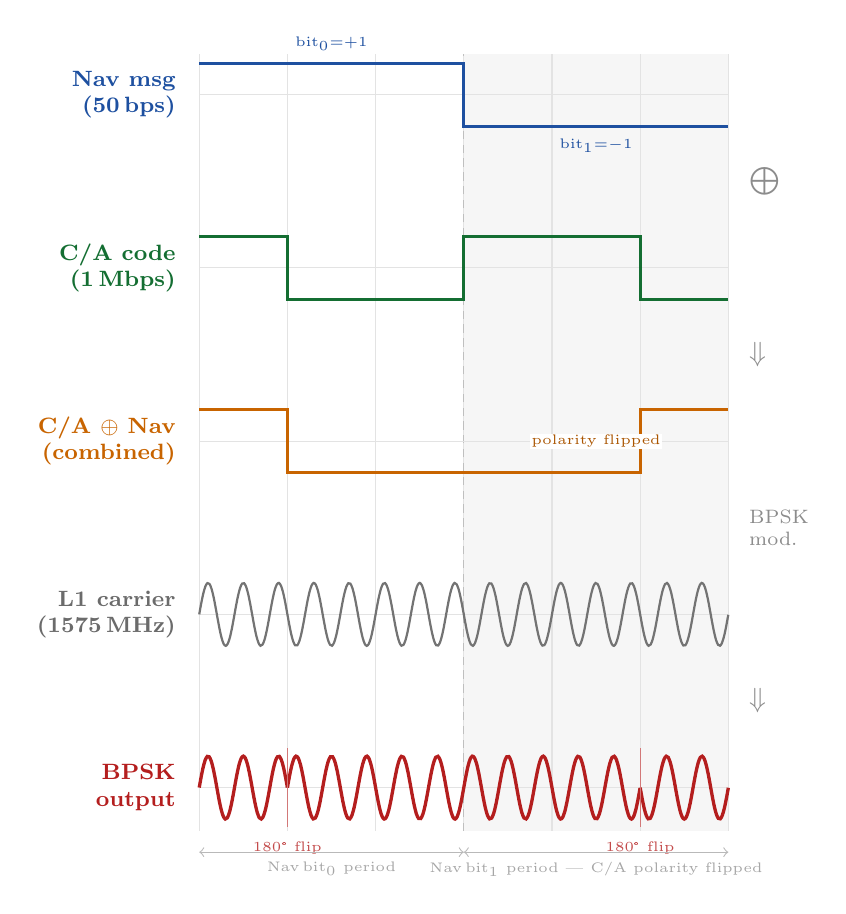
\begin{tikzpicture}[x=1.12cm, y=1.0cm]

  % ── Layout ──────────────────────────────────────────────────────────
  \def\h{0.40}    % square-wave half-height
  \def\amp{0.40}  % sine amplitude

  % Track centres (y)
  \def\yN{8.8}    % Navigation Message
  \def\yCA{6.6}   % C/A code
  \def\yCB{4.4}   % Combined (XOR)
  \def\yL{2.2}    % L1 carrier
  \def\yBP{0.0}   % BPSK output

  % Signal patterns (6 chips, 3 per Nav bit):
  %   C/A:  +1, -1, -1, +1, +1, -1
  %   Nav:  +1, +1, +1, -1, -1, -1  (bit0 x=0..3, bit1 x=3..6)
  %   XOR:  +1, -1, -1, -1, -1, +1  (flipped in bit1 region)

  % ── Nav bit 1 region background shade ───────────────────────────────
  \fill[gray!7] (3, \yBP-0.55) rectangle (6, \yN+0.52);

  % ── Chip boundary gridlines ──────────────────────────────────────────
  \foreach \x in {0,1,2,3,4,5,6} {
    \draw[gray!22, thin] (\x, \yBP-0.55) -- (\x, \yN+0.52);
  }
  \draw[gray!50, thin, densely dashed] (3, \yBP-0.55) -- (3, \yN+0.52);

  % ── Baselines ────────────────────────────────────────────────────────
  \foreach \yy in {\yN, \yCA, \yCB, \yL, \yBP} {
    \draw[gray!22, thin] (0,\yy) -- (6,\yy);
  }

  % ── Row labels ───────────────────────────────────────────────────────
  \node[left=5pt, font=\footnotesize\bfseries, color=keyblue, align=right]
    at (0,\yN) {Nav msg\\(50\,bps)};
  \node[left=5pt, font=\footnotesize\bfseries, color=defgreen, align=right]
    at (0,\yCA) {C/A code\\(1\,Mbps)};
  \node[left=5pt, font=\footnotesize\bfseries, color=noteorange, align=right]
    at (0,\yCB) {C/A $\oplus$ Nav\\(combined)};
  \node[left=5pt, font=\footnotesize\bfseries, color=black!58, align=right]
    at (0,\yL) {L1 carrier\\(1575\,MHz)};
  \node[left=5pt, font=\footnotesize\bfseries, color=warnred, align=right]
    at (0,\yBP) {BPSK\\output};

  % ── Navigation Message ───────────────────────────────────────────────
  \draw[very thick, color=keyblue]
    (0,\yN+\h) -- (3,\yN+\h) -- (3,\yN-\h) -- (6,\yN-\h);
  \node[font=\tiny, above=1pt, color=keyblue] at (1.5,\yN+\h)
    {$\mathrm{bit}_0{=}{+1}$};
  \node[font=\tiny, below=1pt, color=keyblue] at (4.5,\yN-\h)
    {$\mathrm{bit}_1{=}{-1}$};

  % ── C/A code: +1,-1,-1,+1,+1,-1 ────────────────────────────────────
  \draw[very thick, color=defgreen]
    (0,\yCA+\h) -- (1,\yCA+\h)
    -- (1,\yCA-\h) -- (3,\yCA-\h)
    -- (3,\yCA+\h) -- (5,\yCA+\h)
    -- (5,\yCA-\h) -- (6,\yCA-\h);

  % ── Combined (XOR): +1,-1,-1,-1,-1,+1 ───────────────────────────────
  \draw[very thick, color=noteorange]
    (0,\yCB+\h) -- (1,\yCB+\h)
    -- (1,\yCB-\h) -- (5,\yCB-\h)
    -- (5,\yCB+\h) -- (6,\yCB+\h);
  % "flipped" label in combined track, nav-bit-1 region
  \node[font=\tiny, color=noteorange!85!black, fill=white, inner sep=0.5pt]
    at (4.5,\yCB) {polarity flipped};

  % ── Operation labels on right ────────────────────────────────────────
  \node[right=4pt, font=\normalsize, color=black!45] at (6, 7.7) {$\bigoplus$};
  \node[right=4pt, font=\normalsize, color=black!45] at (6, 5.5) {$\Downarrow$};
  \node[right=4pt, font=\scriptsize, color=black!45, align=left] at (6, 3.3)
    {BPSK\\mod.};
  \node[right=4pt, font=\normalsize, color=black!45] at (6, 1.1) {$\Downarrow$};

  % ── L1 carrier (2.5 cycles per chip = sin(900° × x)) ─────────────────
  \draw[thick, color=black!55, domain=0:6, samples=260, smooth]
    plot (\x, {\yL + \amp*sin(900*\x)});

  % ── BPSK output ──────────────────────────────────────────────────────
  % XOR pattern: +1 (chip 0), -1 (chips 1-4), +1 (chip 5)
  % Phase flips at x=1 and x=5 (both are zero-crossings of sin(900°x))
  \draw[very thick, color=warnred, domain=0:1, samples=45, smooth]
    plot (\x, {\yBP + \amp*sin(900*\x)});
  \draw[very thick, color=warnred, domain=1:5, samples=165, smooth]
    plot (\x, {\yBP - \amp*sin(900*\x)});
  \draw[very thick, color=warnred, domain=5:6, samples=45, smooth]
    plot (\x, {\yBP + \amp*sin(900*\x)});

  % ── Phase-flip markers ───────────────────────────────────────────────
  \foreach \xf in {1, 5} {
    \draw[thin, warnred!60] (\xf, \yBP-0.50) -- (\xf, \yBP+0.50);
    \node[below=2pt, font=\tiny, color=warnred!80] at (\xf, \yBP-0.50)
      {180° flip};
  }

  % ── Period labels at bottom ──────────────────────────────────────────
  \draw[<->, thin, gray!55] (0,\yBP-0.82) -- (3,\yBP-0.82)
    node[midway, below, font=\tiny, color=gray!70] {Nav\,$\mathrm{bit}_0$ period};
  \draw[<->, thin, gray!55] (3,\yBP-0.82) -- (6,\yBP-0.82)
    node[midway, below, font=\tiny, color=gray!70]
      {Nav\,$\mathrm{bit}_1$ period --- C/A polarity flipped};

\end{tikzpicture}
\caption{How the GPS signal is built up layer by layer.
  \textbf{Blue}: Navigation Message (slow data bits, 50\,bps) — long
  rectangles showing bit$_0{=}+1$ then bit$_1{=}-1$.
  \textbf{Green}: C/A ranging code (fast pseudorandom chips, 1\,Mbps).
  \textbf{Orange}: XOR-combined signal --- identical to C/A during bit$_0$,
  but with every chip polarity flipped during bit$_1$ (shaded region).
  \textbf{Grey}: L1 carrier sine wave (schematic; real frequency
  $\approx$\,1540$\times$ the C/A chip rate).
  \textbf{Red}: final BPSK broadcast signal --- the carrier with 180°
  phase flips wherever the combined signal is $-1$.
  The receiver decodes the signal in two steps: (1) autocorrelate to find
  C/A lock and extract timing; (2) track polarity flips to read Nav bits.}
\end{figure}

\begin{notebox}
  \textbf{Why a pseudorandom C/A code?}

  The C/A code is a specific sequence of 1023 chips (bits) chosen for its
  excellent autocorrelation properties: when you multiply the sequence
  by a time-shifted version of itself and sum the result, you get a large
  spike only when the two copies are perfectly aligned, and near-zero
  otherwise.
  This is the mechanism the receiver uses to measure time-of-flight.

  Every satellite broadcasts a \emph{different} C/A code
  (there are 1023 distinct codes, one assigned to each satellite ID).
  This means all satellites can transmit on the same L1 frequency
  simultaneously without interfering --- a technique called
  \textbf{CDMA} (Code Division Multiple Access).
  Your receiver knows which codes belong to which satellites and can tune
  into each one independently.
\end{notebox}

\begin{figure}[H]
  \centering
  
\includegraphics[width=0.82\textwidth]{slide-24.jpg}
  \caption{Signal reception by autocorrelation.  The receiver generates a
    local replica of the C/A code, driven by its own clock $T$.
    It slides the replica in time until the autocorrelation with the incoming
    signal peaks at $+1$.
    The time shift at the peak is $T - T^s$, the clock difference used to
    compute the pseudorange.}
\end{figure}
The receiver cannot simply look at a waveform and read off a timestamp ---
the signal has no pulse or edge to identify.
Instead it uses \textbf{autocorrelation}:

\begin{enumerate}[leftmargin=1.5em, itemsep=3pt]
  \item The receiver generates a local \textbf{replica} of the satellite's
    C/A code, running on its own (imperfect) clock $T$.
  \item It multiplies the received signal by the replica bit by bit and sums
    the result.
\end{enumerate}
\subsubsection*{How the receiver measures arrival time}

The receiver does \emph{not} receive a pre-made copy of the C/A code ---
it \textbf{generates one locally from scratch}.
Every GPS receiver contains the algorithm and the code table for every
satellite, so it can reproduce any satellite's 1023-chip sequence
internally at any time.

The received signal has the satellite's C/A code embedded in it, but that
code started being transmitted at the satellite's clock time $T^s$.
The receiver's local replica starts from its own clock time $T$.
Those two clocks are offset by an unknown amount $\Delta t = T - T^s$, so
the two copies of the code are \emph{shifted} relative to each other by
exactly $\Delta t$.

The receiver tries different lag values $k$ --- asking ``what if I delay
my replica by $k$ chips?'' --- and for each $k$ computes the
\textbf{cross-correlation}:
\[
  R(k) = \frac{1}{N}\sum_{i=0}^{N-1} x_i \cdot y_{i-k}
\]
where $x_i$ is the received chip and $y_{i-k}$ is the local replica
delayed by $k$ chips.
This is exactly the lag-$k$ correlation from signal processing:

\begin{itemize}[leftmargin=1.5em, itemsep=3pt]
  \item \textbf{$k \neq \Delta t$:} the two pseudorandom sequences are
    misaligned.
    Half the products are $(+1)\times(-1) = -1$ and half are
    $(+1)\times(+1) = +1$ --- they nearly cancel, so $R(k) \approx 0$.
  \item \textbf{$k = \Delta t$:} the sequences line up perfectly.
    Every chip multiplies its own copy, so every product $= +1$, giving
    $R(\Delta t) = +1$.
\end{itemize}

There is a single sharp spike in $R$ at exactly one lag value and
near-zero everywhere else.
The receiver scans through trial lags (or uses a \emph{delay-locked loop}
to continuously track the peak) until it finds that spike.
The lag $k$ where $R(k) = 1$ is the answer:
\[
  \Delta t = k \qquad \Rightarrow \qquad \rho = c\,\Delta t
\]

The autocorrelation is therefore exactly what tells the receiver:
\emph{``the two signals are fully correlated at lag $k$ --- so the signal
must have taken time $k$ to travel from the satellite to me.''}

\begin{notebox}
  \textbf{Connection to Games-on-Track chirp (Section~1)}

  This is the same cross-correlation timestamping principle used by the
  radio chirp system.
  Instead of a swept frequency, GPS uses a pseudorandom binary code.
  Both work on the same idea: transmit a known pattern, generate a local
  copy, slide it in time until the two match --- the required shift is the
  travel time.
  The C/A code's 1023-chip pseudorandom structure is chosen specifically
  because it produces a very sharp, unambiguous autocorrelation spike with
  near-zero sidelobes, making the timing measurement clean and precise.
\end{notebox}

% ── Key takeaways ─────────────────────────────────────────────────────────────
\begin{keybox}
  \textbf{Section 3 --- Key Takeaways}
  \begin{itemize}[leftmargin=1.2em,itemsep=2pt]
    \item The measured quantity is the \textbf{pseudorange}
      $\rho = c\Delta t = r + c\tau$, where $r$ is true range and $\tau$ is
      receiver clock error.
      Satellite clock error is correctable from the Navigation Message;
      $\tau$ is solved alongside $(x,y,z)$ using four satellites.
    \item GPS has four segments: \textbf{Space} (satellites), \textbf{Control}
      (ground monitoring, orbit/clock corrections), \textbf{User} (receivers),
      \textbf{Ground} (tracking reference networks).
    \item Each satellite carries redundant \textbf{atomic clocks}; the Control
      Segment monitors health and uploads Keplerian updates hourly.
    \item Receivers output \textbf{NMEA sentences} (e.g.\ \$GPGGA) --- plain
      ASCII with position, time, altitude, DOP, and satellite count.
    \item The \textbf{Navigation Message} (50\,bps) carries clock corrections
      (subframe~1), precise \emph{ephemeris} for this satellite (subframes 2--3),
      and coarse \emph{almanac} for all satellites (subframes 4--5).
    \item The receiver measures pseudorange via \textbf{autocorrelation}: it
      slides a local C/A code replica until it aligns with the incoming signal;
      the required time shift is $\Delta t = T - T^s$.
      Different satellites use different C/A codes on the same frequency
      (\textbf{CDMA}).
  \end{itemize}
\end{keybox}

% ==============================================================================
\clearpage
\section*{Section 4 \quad GPS Position Estimation}
% ==============================================================================

We now have all the pieces: satellites with known ECEF positions, pseudorange
measurements from each, and the understanding that those measurements are
corrupted by the receiver clock error $\tau$.
This section shows how to go from a set of pseudoranges to an estimated
receiver position --- and how to quantify how uncertain that estimate is.

% ------------------------------------------------------------------------------
\subsection*{4.1 \quad The Pseudorange Observation Equation}
% ------------------------------------------------------------------------------

\begin{figure}[H]
  \centering
  
\includegraphics[width=0.78\textwidth]{slide-25.jpg}
  \caption{Full pseudorange model incorporating both the receiver clock bias
    $\tau$ and the satellite clock bias $\tau_S$.
    The satellite transmits its position and $\tau_S$; the receiver solves
    for its own position and its unknown $\tau$.}
\end{figure}

The raw measurement is the pseudorange $P_S$, computed from the time
difference between transmission and reception:
\[
  P_S = (T - T_S)\,c
\]
Both clocks deviate from true GPS time.
Substituting $T = t + \tau$ (receiver) and $T_S = t_S + \tau_S$ (satellite):
\[
  P_S = \bigl[(t+\tau) - (t_S+\tau_S)\bigr]\,c
      = \underbrace{c(t - t_S)}_{\rho(t,\,t_S)} + c\tau - c\tau_S
\]
so the pseudorange is:
\[
  \boxed{P_S = \rho(t,\,t_S) + c\tau - c\tau_S}
\]

\begin{center}
\begin{tabular}{@{} l p{2.8cm} p{8.2cm} @{}}
  \toprule
  Symbol & Name & Meaning \\
  \midrule
  $P_S$ & Pseudorange &
    The measured apparent distance: raw time difference $\times\,c$.
    ``Pseudo'' because it includes clock offsets. \\
  $\rho(t,t_S)$ & True geometric range &
    Actual Euclidean distance from receiver to satellite:
    $\sqrt{(x_S{-}x)^2 + (y_S{-}y)^2 + (z_S{-}z)^2}$. \\
  $\tau$ & Receiver clock error &
    Offset of the receiver's quartz oscillator from true GPS time.
    \textbf{Unknown} --- must be estimated alongside position. \\
  $\tau_S$ & Satellite clock error &
    Offset of the satellite's atomic clock from true GPS time.
    \textbf{Known} --- provided in the Navigation Message as a polynomial;
    $c\tau_S$ is subtracted before further processing. \\
  $t$ & True reception time & True GPS time when signal arrives at receiver. \\
  $t_S$ & True transmission time & True GPS time when satellite sent the signal. \\
  \bottomrule
\end{tabular}
\end{center}

\begin{notebox}
  \textbf{What are the unknowns?}

  After correcting the known satellite clock term, the corrected pseudorange is:
  \[
    \tilde{P}_S = P_S + c\tau_S = \rho(t,\,t_S) + c\tau
  \]
  The satellite position $(x_S, y_S, z_S)$ at time $t_S$ is known from the
  ephemeris (Section~2.4), so $\rho$ contains three unknowns: the receiver
  coordinates $x(t),\,y(t),\,z(t)$.
  Plus the fourth unknown $\tau$, the receiver clock error.

  \textbf{4 unknowns, 1 equation per satellite} --- need at least 4 satellites
  for a unique solution.
  This is the same ``why 4 satellites?'' conclusion from Section~2.1, now
  seen as a proper equation system.

  Atmospheric delays (ionospheric and tropospheric signal slowing) and
  relativistic effects are real but are omitted here for simplicity;
  operational receivers apply models to correct for both.
\end{notebox}

% ------------------------------------------------------------------------------
\subsection*{4.2 \quad Linearising for Multiple Satellites}
% ------------------------------------------------------------------------------

\begin{figure}[H]
  \centering
  
\includegraphics[width=0.82\textwidth]{slide-26.jpg}
  \caption{With $m \geq 4$ satellites the $m$ pseudorange equations are
    stacked and linearised around an initial guess, giving the linear
    system $b = A\hat{\xi} + \nu$.}
\end{figure}

With $m$ satellites the corrected equations are:
\[
  \tilde{P}_k = \rho_k(x,y,z,t_k) + c\tau, \qquad k = 1,\dots,m
\]
Each $\rho_k$ is a square root of squared differences ---
the system is \textbf{nonlinear} in the unknowns $(x,y,z,\tau)$.

The standard approach: linearise around an initial guess
$(x_0,y_0,z_0,\tau_0)$ using a first-order Taylor expansion, exactly as
in the Jacobian linearisation from Lecture~7.
Let $P_{0,k}$ be the predicted pseudorange to satellite $k$ at the initial
guess.
Define the \textbf{correction vector} $\hat{\xi}$ and
\textbf{measurement-difference vector} $b$:
\[
  \hat{\xi} =
  \begin{bmatrix} x - x_0 \\ y - y_0 \\ z - z_0 \\ \tau - \tau_0
  \end{bmatrix}, \qquad
  b =
  \begin{bmatrix} \tilde{P}_1 - P_{0,1} \\ \tilde{P}_2 - P_{0,2} \\
    \vdots \\ \tilde{P}_m - P_{0,m}
  \end{bmatrix}
\]
Stacking all $m$ equations gives:
\[
  b = A\hat{\xi} + \nu
\]
Here $b$ contains the \emph{known} numbers --- what you measured minus what
you predicted --- and $A$ is the $m \times 4$ Jacobian (defined below).
$\nu$ is the \textbf{fit residual} --- the leftover mismatch after
subtracting the model's prediction $A\hat{\xi}$ from $b$:
\[
  \nu = b - A\hat{\xi}
\]
To be clear on the difference:
\begin{itemize}[leftmargin=1.5em, itemsep=2pt]
  \item $b_k = \tilde{P}_k - P_{0,k}$: how far the \emph{observed}
    pseudorange is from what the initial guess predicted.
    This is \emph{computed from data} and is the input to the problem.
  \item $\nu_k = b_k - (A\hat{\xi})_k$: how far the fitted model still
    misses the data after the best $\hat{\xi}$ is found.
    This is what the fit \emph{cannot explain} --- due to measurement noise
    and the truncated higher-order Taylor terms.
\end{itemize}
In a perfect, noiseless, linear world $\nu = \mathbf{0}$ and
$b = A\hat{\xi}$ exactly.
In practice $\nu \neq \mathbf{0}$; least squares finds the $\hat{\xi}$
that makes $\|\nu\|^2$ as small as possible.
The $m \times 4$ Jacobian $A$ is:
\[
  A =
  \begin{bmatrix}
    \dfrac{\partial P_1}{\partial x} & \dfrac{\partial P_1}{\partial y} &
    \dfrac{\partial P_1}{\partial z} & \dfrac{\partial P_1}{\partial\tau}
    \\[8pt]
    \vdots & \vdots & \vdots & \vdots \\[4pt]
    \dfrac{\partial P_m}{\partial x} & \dfrac{\partial P_m}{\partial y} &
    \dfrac{\partial P_m}{\partial z} & \dfrac{\partial P_m}{\partial\tau}
  \end{bmatrix}
\]

\begin{notebox}
  \textbf{What are the partial derivatives in $A$?}

  The first three columns of each row are the partial derivatives of
  $\rho_k$ with respect to receiver position:
  \[
    \frac{\partial P_k}{\partial x}
      = -\frac{x_S^{(k)} - x_0}{\rho_{0,k}}, \quad
    \frac{\partial P_k}{\partial y}
      = -\frac{y_S^{(k)} - y_0}{\rho_{0,k}}, \quad
    \frac{\partial P_k}{\partial z}
      = -\frac{z_S^{(k)} - z_0}{\rho_{0,k}}
  \]
  These are the \emph{direction cosines} from the initial receiver guess to
  satellite $k$ --- the components of the unit vector pointing from receiver
  toward the satellite.
  Physically: moving the receiver by a small step in $x$ changes the range
  to satellite $k$ only by the projection of that step onto the
  receiver-to-satellite direction.

  The fourth column is simply $c$ for every satellite:
  \[
    \frac{\partial P_k}{\partial \tau} = c
  \]
  because a clock offset $\delta\tau$ adds the same $c\,\delta\tau$ to
  every pseudorange, regardless of which satellite.

  So each row of $A$ looks like:
  \[
    \begin{bmatrix}
      -\dfrac{x_S^{(k)}-x_0}{\rho_{0,k}} &
      -\dfrac{y_S^{(k)}-y_0}{\rho_{0,k}} &
      -\dfrac{z_S^{(k)}-z_0}{\rho_{0,k}} & c
    \end{bmatrix}
  \]
  a unit vector pointing toward the satellite, with $c$ appended.
\end{notebox}

% ------------------------------------------------------------------------------
\subsection*{4.3 \quad Least-Squares Solution}
% ------------------------------------------------------------------------------

\begin{figure}[H]
  \centering
  
\includegraphics[width=0.72\textwidth]{slide-27.jpg}
  \caption{With $m > 4$ satellites the system is overdetermined.
    Least squares finds $\hat{\xi}$ that minimises the total squared
    residual across all pseudorange measurements.}
\end{figure}

With $m > 4$ satellites the system $b = A\hat{\xi} + \nu$ is
\textbf{overdetermined} --- more equations than unknowns.
There is no exact solution; instead minimise the sum of squared residuals:
\[
  J(\hat{\xi}) = \nu^\top\nu = (b - A\hat{\xi})^\top(b - A\hat{\xi})
\]
Setting $\partial J/\partial\hat{\xi} = 0$ gives the
\textbf{normal equation} (same structure as the disc-fitting solution in
Lecture~7):
\[
  \boxed{\hat{\xi} = (A^\top A)^{-1} A^\top b}
\]

\begin{notebox}
  \textbf{Why more satellites help, and why geometry matters}

  With exactly 4 satellites you get an exact solution --- but any noise on
  a pseudorange goes straight into your position error with nothing to
  average it out.
  With 5 or more satellites the extra measurements are redundant but
  \emph{useful}: least squares finds the single $(x,y,z,\tau)$ that best
  fits all measurements simultaneously, averaging out random noise.

  \textbf{Why $m \geq 5$ in practice:}
  $A^\top A$ must be invertible, meaning the 4 columns of $A$ must be
  linearly independent.
  This fails if all satellites happen to be coplanar with the receiver ---
  their direction-cosine rows would lie in the same 3D subspace.
  With 5 or more well-spread satellites this is essentially impossible.

  \textbf{DOP revisited:} the conditioning of $A^\top A$ is exactly what
  DOP quantifies (Section~3.3).
  Good satellite spread → $A^\top A$ well-conditioned →
  $(A^\top A)^{-1}$ small → measurement noise produces small position
  errors (low DOP).
  Poor spread → $A^\top A$ nearly singular → same noise causes large
  errors (high DOP).
\end{notebox}

% ------------------------------------------------------------------------------
\subsection*{4.4 \quad Error Propagation and Covariance}
% ------------------------------------------------------------------------------

\begin{figure}[H]
  \centering
  
\includegraphics[width=0.78\textwidth]{slide-28.jpg}
  \caption{Propagating pseudorange measurement noise $\Sigma_\nu$ through
    the least-squares formula gives the position covariance $\Sigma_\xi$.}
\end{figure}

The estimation error (how far $\hat{\xi}$ is from the true solution)
propagates from measurement noise $\nu$ as:
\[
  \nu_\xi = \hat{\xi} - \xi_\text{true} = (A^\top A)^{-1} A^\top \nu
\]
Taking the expectation of the outer product gives the
\textbf{covariance matrix of position errors}:
\[
  \Sigma_\xi = (A^\top A)^{-1} A^\top \,\Sigma_\nu\, A\,(A^\top A)^{-1}
\]

\begin{notebox}
  \textbf{The equal-noise special case --- what the diagonal gives you}

  The assumption $\Sigma_\nu = \sigma_\nu^2 I$ is a statement about the
  \textbf{$m$ pseudorange measurements} (not the 4 unknowns).
  It says two things simultaneously:
  \begin{itemize}[leftmargin=1.5em, itemsep=1pt]
    \item \emph{Same noise on every satellite:} every pseudorange has the
      same variance $\sigma_\nu^2$, regardless of which satellite it comes
      from (elevation angle, signal strength, atmospheric path length,
      etc.).
    \item \emph{Independent between satellites:} the noise on one
      satellite's measurement is unrelated to the noise on another's ---
      the off-diagonals of $\Sigma_\nu$ are zero.
  \end{itemize}
  In reality neither is perfectly true --- a satellite near the horizon
  has its signal travel through much more atmosphere and is typically
  noisier.
  The general formula $\Sigma_\xi = (A^\top A)^{-1}A^\top\Sigma_\nu A
  (A^\top A)^{-1}$ handles unequal noise by weighting satellites
  differently.
  The equal-noise case is a simplification that gives a clean result:
  \[
    \Sigma_\xi = \sigma_\nu^2\,(A^\top A)^{-1}
  \]
  This means the \emph{shape} and \emph{size} of the uncertainty ellipsoid
  is entirely determined by the satellite geometry $(A^\top A)^{-1}$;
  the noise level $\sigma_\nu^2$ just scales the whole thing up or down
  uniformly.
  Poor geometry amplifies noise; good geometry suppresses it.

  The \textbf{diagonal elements} of $\Sigma_\xi$ are the individual
  variances (squared 1-sigma errors):
  \begin{itemize}[leftmargin=1.5em, itemsep=1pt]
    \item $[\Sigma_\xi]_{11} = \sigma_x^2$ --- variance of $x$-coordinate
      error
    \item $[\Sigma_\xi]_{22} = \sigma_y^2$ --- variance of $y$-coordinate
      error
    \item $[\Sigma_\xi]_{33} = \sigma_z^2$ --- variance of $z$-coordinate
      error
    \item $[\Sigma_\xi]_{44} = \sigma_\tau^2$ --- variance of receiver
      clock-error estimate
  \end{itemize}
  The \textbf{off-diagonal elements} describe cross-correlations: e.g.\
  whether an overestimate of $x$ tends to come with an overestimate of $y$.
\end{notebox}

% ------------------------------------------------------------------------------
\subsection*{4.5 \quad Uncertainty Ellipsoid in Local NEU Coordinates}
% ------------------------------------------------------------------------------

\begin{figure}[H]
  \centering
  
\includegraphics[width=0.72\textwidth]{slide-29.jpg}
  \caption{The ECEF covariance $\Sigma_\xi$ is rotated into the local
    North-East-Up frame at the receiver's latitude $\phi$ and longitude
    $\lambda$ using $R_{\phi\lambda}$.}
\end{figure}

The covariance $\Sigma_\xi$ describes errors in ECEF $(x,y,z)$ coordinates.
An error of 5\,m in the ECEF $x$-direction is hard to interpret ---
it could mean northward, eastward, or upward depending on where on Earth
you are.
The solution is to rotate the error ellipsoid into the local
\textbf{North-East-Up} frame at the receiver's position
(introduced in Section~2.3).
This rotation depends only on \textbf{where on Earth the receiver is} ---
specifically its latitude $\phi$ and longitude $\lambda$ (the same
$\phi, \lambda$ from Section~2.2).
Once you have a GPS fix you know your approximate $\phi$ and $\lambda$,
and you use those to build the rotation matrix.

The rotation matrix from ECEF to NEU at latitude $\phi$,
longitude $\lambda$ is:
\[
  R_{\phi\lambda} =
  \begin{bmatrix}
    -\sin\phi\cos\lambda & -\sin\phi\sin\lambda &  \cos\phi \\
    -\sin\lambda         &  \cos\lambda         &  0        \\
     \cos\phi\cos\lambda &  \cos\phi\sin\lambda &  \sin\phi
  \end{bmatrix}
\]

The position error and its covariance in local NEU coordinates are:
\[
  \nu_\text{NEU} = R_{\phi\lambda}\,\nu_\xi, \qquad
  \boxed{\Sigma_\text{NEU} = R_{\phi\lambda}\,\Sigma_\xi\,R_{\phi\lambda}^\top}
\]

\begin{notebox}
  \textbf{Reading the NEU covariance}

  The three rows of $R_{\phi\lambda}$ are the unit vectors pointing
  North, East, and Up from the observer's location:
  \begin{itemize}[leftmargin=1.5em, itemsep=2pt]
    \item \textbf{Row 1 (North):}
      $[-\sin\phi\cos\lambda,\;-\sin\phi\sin\lambda,\;\cos\phi]$ ---
      points toward the geographic north pole.
    \item \textbf{Row 2 (East):}
      $[-\sin\lambda,\;\cos\lambda,\;0]$ ---
      lies in the equatorial plane, pointing east.
    \item \textbf{Row 3 (Up):}
      $[\cos\phi\cos\lambda,\;\cos\phi\sin\lambda,\;\sin\phi]$ ---
      points radially outward from Earth's centre.
  \end{itemize}

  After the rotation, the diagonal of $\Sigma_\text{NEU}$ is immediately
  readable:
  \begin{itemize}[leftmargin=1.5em, itemsep=1pt]
    \item $[\Sigma_\text{NEU}]_{11} = \sigma_N^2$ --- north variance
    \item $[\Sigma_\text{NEU}]_{22} = \sigma_E^2$ --- east variance
    \item $[\Sigma_\text{NEU}]_{33} = \sigma_U^2$ --- vertical (up)
      variance
  \end{itemize}
  Horizontal uncertainty: $\sigma_H = \sqrt{\sigma_N^2 + \sigma_E^2}$.

  \textbf{Why vertical error is larger:}
  all GPS satellites are above the horizon --- there is no satellite
  directly below the receiver.
  The Up direction is poorly constrained compared to North and East,
  so $\sigma_U$ is typically 2--3$\times$ larger than $\sigma_H$.
  This is a fundamental geometric limitation of GPS, not a hardware
  imperfection.
\end{notebox}

% ── Key takeaways ─────────────────────────────────────────────────────────────
\begin{keybox}
  \textbf{Section 4 --- Key Takeaways}
  \begin{itemize}[leftmargin=1.2em,itemsep=2pt]
    \item The pseudorange model:
      $P_S = \rho(t,t_S) + c\tau - c\tau_S$.
      Correcting the known $c\tau_S$ leaves 4 unknowns:
      $(x, y, z, \tau)$.
    \item The nonlinear equations are \textbf{linearised} around a guess,
      giving $b = A\hat{\xi} + \nu$.
      Each row of $A$ is a unit vector toward one satellite
      (direction cosines), with $c$ appended for the clock column.
    \item \textbf{Least squares:}
      $\hat{\xi} = (A^\top A)^{-1}A^\top b$.
      Requires $A^\top A$ non-singular (satellites not coplanar);
      $m \geq 5$ gives a robust overdetermined solution.
    \item \textbf{DOP} is the conditioning of $A^\top A$: poor geometry
      → large $(A^\top A)^{-1}$ → measurement noise amplified into large
      position errors.
    \item \textbf{Covariance:}
      $\Sigma_\xi = \sigma_\nu^2(A^\top A)^{-1}$.
      Diagonal = individual variances for $x,y,z,\tau$.
    \item Rotating to local NEU via
      $\Sigma_\text{NEU} = R_{\phi\lambda}\Sigma_\xi R_{\phi\lambda}^\top$
      gives interpretable uncertainties.
      Vertical error is $\approx$\,2--3$\times$ horizontal due to no
      satellites below the horizon.
  \end{itemize}
\end{keybox}

% ==============================================================================
\clearpage
\section*{Section 5 \quad Tracking Moving Targets}
% ==============================================================================

\begin{figure}[H]
  \centering
  
\includegraphics[width=0.82\textwidth]{slide-30.jpg}
  \caption{Block diagram of the Kalman filter for GPS-based tracking.
    GPS pseudoranges provide noisy position observations $\xi_k$ (via the
    least-squares solution from Section~4).
    The Kalman filter combines these with a constant-velocity motion model
    to estimate both position \emph{and} velocity.}
\end{figure}

So far GPS has been treated as a static problem: estimate the receiver's
position at one instant from one batch of pseudoranges.
In practice the receiver is often \emph{moving} --- a phone, a car, a drone
--- and we want to track its position and velocity continuously over time.

The solution is a \textbf{Kalman filter} applied to consecutive GPS
observations.
This connects directly to the state-space estimation framework from the
Kalman filter lectures: GPS provides the observations, and a motion model
provides the prediction between observations.

% ------------------------------------------------------------------------------
\subsection*{5.1 \quad State-Space Model}
% ------------------------------------------------------------------------------

The state vector stacks 3D position and 3D velocity into six components:
\[
  \chi_k =
  \begin{bmatrix}
    x_k \\ y_k \\ z_k \\ v_{x,k} \\ v_{y,k} \\ v_{z,k}
  \end{bmatrix}
\]

\textbf{State transition matrix $\Phi$} (how the state evolves from step
$k$ to $k+1$, assuming constant velocity and sample period $T_s$):
\[
  \Phi =
  \begin{bmatrix}
    1 & 0 & 0 & T_s & 0   & 0   \\
    0 & 1 & 0 & 0   & T_s & 0   \\
    0 & 0 & 1 & 0   & 0   & T_s \\
    0 & 0 & 0 & 1   & 0   & 0   \\
    0 & 0 & 0 & 0   & 1   & 0   \\
    0 & 0 & 0 & 0   & 0   & 1
  \end{bmatrix}
\]

\textbf{Observation matrix $H$} (GPS measures position, not velocity):
\[
  H = \bigl[I \quad 0\bigr] \in \mathbb{R}^{3\times 6}
\]

\begin{notebox}
  \textbf{What $\Phi$ and $H$ say about the model}

  \textbf{$\Phi$ encodes a constant-velocity motion model.}
  Read it row by row:
  \begin{itemize}[leftmargin=1.5em, itemsep=2pt]
    \item \emph{Top-left $3\times3$ identity:} position at the next step
      starts from current position.
    \item \emph{Top-right $3\times3$ block with $T_s$ on the diagonal:}
      position is updated by adding velocity $\times$ time step
      ($x_{k+1} = x_k + T_s\,v_{x,k}$, and similarly for $y$ and $z$).
    \item \emph{Bottom-left $3\times3$ zeros:} velocity does not depend
      on current position.
    \item \emph{Bottom-right $3\times3$ identity:} velocity is assumed
      constant between steps ($v_{x,k+1} = v_{x,k}$).
  \end{itemize}
  Real acceleration (turning, braking) is not modelled explicitly ---
  it is absorbed into the \textbf{process noise} $w_k$.
  If the target accelerates more than $w_k$ accounts for, the filter
  lags behind until the GPS observations pull the estimate back.

  \textbf{$H = [I \quad 0]$} means the GPS measurement gives you the
  first three state components (position $x, y, z$) but tells you
  nothing directly about velocity.
  The Kalman filter infers velocity from the \emph{change} in position
  over consecutive GPS fixes.
\end{notebox}

% ------------------------------------------------------------------------------
\subsection*{5.2 \quad Applying the Kalman Filter}
% ------------------------------------------------------------------------------

The complete discrete-time model is:
\[
  \chi_{k+1} = \Phi\,\chi_k + w_k \qquad \text{(process / motion model)}
\]
\[
  \xi_k = H\,\chi_k + \nu_k \qquad \text{(observation model)}
\]
where $w_k$ and $\nu_k$ are zero-mean Gaussian noise:
\begin{itemize}[leftmargin=1.5em, itemsep=2pt]
  \item $w_k \sim \mathcal{N}(0, Q)$: process noise covariance $Q$
    captures unmodelled accelerations.
  \item $\nu_k \sim \mathcal{N}(0, R)$: observation noise covariance $R$
    is the GPS position error covariance.
\end{itemize}

\begin{notebox}
  \textbf{Where does the observation noise covariance $R$ come from?}

  This is exactly $\Sigma_\text{NEU}$ (or $\Sigma_\xi$ restricted to the
  position components) from Section~4.
  The full GPS covariance analysis --- pseudorange noise propagated through
  the least-squares formula and rotated into local NEU coordinates ---
  directly gives you $R$ for the Kalman filter.
  The two sections are connected: Section~4 produces the measurement
  uncertainty; Section~5 plugs it into the filter.

  In practice $R$ changes from epoch to epoch as the satellite geometry
  changes (different satellites come into and out of view), so a GPS/Kalman
  system recomputes $R$ at each time step.
\end{notebox}

The standard Kalman predict-update cycle then runs at each GPS epoch:
\begin{enumerate}[leftmargin=1.5em, itemsep=3pt]
  \item \textbf{Predict:} propagate the state estimate and its covariance
    forward using $\Phi$.
  \item \textbf{Update:} take the new GPS pseudoranges, compute the
    least-squares position fix $\hat{\xi}_k$ (Section~4), and correct the
    predicted state toward the observation.
  \item The Kalman gain balances trust in the motion model vs.\ trust in
    the GPS measurement, weighted by their respective covariances $Q$
    and $R$.
\end{enumerate}

The output at each step is an estimate of \emph{both} position and
velocity, smoother than raw GPS alone because the filter integrates
information across multiple time steps.

% ── Key takeaways ─────────────────────────────────────────────────────────────
\begin{keybox}
  \textbf{Section 5 --- Key Takeaways}
  \begin{itemize}[leftmargin=1.2em,itemsep=2pt]
    \item A \textbf{Kalman filter} wraps around the GPS least-squares
      solver to track moving receivers continuously, estimating both
      position and velocity.
    \item The \textbf{state vector} is
      $\chi_k = [x,y,z,v_x,v_y,v_z]^\top$;
      the \textbf{constant-velocity model} gives $\Phi$ (position updated
      by $v \cdot T_s$, velocity held constant).
    \item GPS observes only position: $H = [I\;\; 0]$.
      Velocity is inferred from position changes over time.
    \item The GPS observation noise covariance $R$ comes directly from
      Section~4's covariance analysis ($\Sigma_\xi$ or $\Sigma_\text{NEU}$)
      and is recomputed each epoch as satellite geometry changes.
    \item Unmodelled accelerations are absorbed by the process noise $Q$.
  \end{itemize}
\end{keybox}

% ==============================================================================
\clearpage
\section*{Lecture Summary}
% ==============================================================================

\begin{figure}[H]
  \centering
  
\includegraphics[width=0.72\textwidth]{slide-31.jpg}
  \caption{Lecture 8 summary slide.}
\end{figure}

\begin{keybox}
  \textbf{Lecture 8 --- Complete Summary}
  \begin{itemize}[leftmargin=1.2em,itemsep=3pt]
    \item \textbf{Trilateration-based sensors} estimate position from
      range measurements to known anchors.
      Range is obtained via time-of-flight (chirp, acoustic) or signal
      strength (BLE RSSI), depending on hardware constraints.

    \item \textbf{GPS} is a satellite-based trilateration system
      operational since the 1980s.
      Each satellite broadcasts a timing signal and navigation data;
      the receiver uses the signal travel time to compute pseudoranges.

    \item \textbf{Key variables transmitted by each satellite:} satellite
      ECEF position (from ephemeris), satellite clock correction
      $\tau_S$, and the C/A ranging code.
      Together these allow the receiver to compute the corrected
      pseudorange $\tilde{P}_k = \rho_k + c\tau$.

    \item \textbf{Position estimation} uses local linearisation (Jacobian)
      and least squares: $\hat{\xi} = (A^\top A)^{-1}A^\top b$.
      Four unknowns $(x, y, z, \tau)$ require at least 4 satellites;
      $m \geq 5$ gives an overdetermined, noise-averaging solution.

    \item \textbf{Error analysis:} $\Sigma_\xi = \sigma_\nu^2(A^\top A)^{-1}$
      gives position uncertainty in ECEF; rotating to local NEU via
      $\Sigma_\text{NEU} = R_{\phi\lambda}\Sigma_\xi R_{\phi\lambda}^\top$
      gives interpretable horizontal and vertical errors.
      Vertical error is $\approx$\,2--3$\times$ horizontal.

    \item \textbf{Moving targets:} a Kalman filter wraps around the GPS
      solver, using the GPS covariance as observation noise $R$ and a
      constant-velocity model as the prediction step.
  \end{itemize}
\end{keybox}

\end{document}

